\documentclass{article}
\usepackage[pdftex]{graphicx,color}
\usepackage[table]{xcolor}
\usepackage{fullpage,palatino,mathpazo,amsmath,amssymb,url}
\usepackage{url,amsmath,amssymb,subfigure,boxedminipage,shadow}
\usepackage{listings}
\usepackage{tabularx,booktabs,hyperref,ifthen}

\usepackage{tikz}

\usetikzlibrary{math} 
\usetikzlibrary{patterns}
\usetikzlibrary{decorations.pathmorphing}
% arrows is deprecated; removing it will take some time
\usetikzlibrary{arrows,arrows.meta,automata,shadows,shapes,shapes.geometric,circuits.logic.US,shapes.gates.logic.US,calc}

\usepackage{mwe} %example-image 

\tikzset{
  >=Stealth, % can't stand the default arrows
  multrectangle/.style={draw, fill=black!5},
  generator/.style={draw,align=center,fill=blue!5,rounded corners, minimum width=15ex, minimum height=8ex},
%  hwblock/.style={draw, rectangle, rounded corners=.3, very thick, fill=black!5, font=\sf, minimum height=5ex,align=center},
  hwblock/.style={draw, rectangle, rounded corners=.3, thick, fill=black!2, drop shadow={shadow xshift=.5ex,shadow yshift=-.5ex}, font=\sf, minimum height=5ex,align=center},
  hwregblock/.style={hwblock, fill=blue!10},
  every circuit symbol/.style={hwblock},
  filteradd/.style={hwblock, circle, minimum height=1ex},
  filtermult/.style={hwblock, minimum height=7ex, regular polygon, regular polygon sides=3, shape border rotate=180, inner sep= .2ex},
  hwbus/.style={very thick,>={Stealth[length=6pt]}},
  hwbuslarge/.style={line width=2pt,>={Stealth[length=7pt]}},
  hwbuswhitebackground/.style={line width=4pt,color=white},
  hwwire/.style={thin, >={Stealth[length=4pt]}  },
  hwword/.style={draw, rectangle, minimum height=3ex},
  bitwidth/.style={font=\scriptsize,blue},
  abitwidth/.style={bitwidth,above},
  bbitwidth/.style={bitwidth,below},
  lbitwidth/.style={bitwidth,left},
  rbitwidth/.style={bitwidth,right},
  flopocoClass/.style={font=\small\tt,draw,align=center,rectangle,fill=blue!5,minimum height=3ex},
  flopocoInfo/.style={font=\small,align=center,rectangle, fill=yellow!50,fill opacity=0.5, text opacity=1,rounded corners=10}
}
% Other colors that could be used consistent
\definecolor{normalbitcolor}{rgb}{0,0,0.5}
\definecolor{normalbitfillcolor}{rgb}{0.8,1,0.8}
\definecolor{signbitcolor}{rgb}{0.5,0,0}
\definecolor{signbitfillcolor}{rgb}{1,0.8,0.8}

% When we refer to a component in the text
%\newcommand{\texthwblock}[1]{\fbox{\small\sf #1}}
% The following is ugly
\newcommand{\texthwblock}[1]{\raisebox{-.8ex}{\scalebox{0.85}{\tikz{\node[hwblock,text height=1.4ex,text depth=.2ex, minimum height=1ex]{#1}}}}}



\newcommand{\bitwidth}[3]{ % coordinate, text, [a|b|l|r]
    \draw[bitwidth,ultra thin] (#1) ++(0.5ex, 0.5ex)  -- ++(-1ex, -1ex) ++(0.5ex, 0.5ex)  node[#3bitwidth] {#2};
} %

% Shifts in shift-and-add figure
\newcommand{\leftbitshift}[2]{ % coordinate, value
    \draw[font=\small, thick, Latex-] (#1) ++(-2ex, 0)  -- ++(3ex,0)  node[right] {#2};
} %

\newcommand{\rightbitshift}[2]{ % coordinate, value
    \draw[font=\small, thick, Latex-] (#1) ++(2ex, 0)  -- ++(-3ex,0)  node[left] {#2};
} %


\newcommand{\vhdlfile}[2]{ % x,y
  \draw[fill=black!5] (#1,#2) ++(3.5ex, -5ex) -- ++(-7ex,0) -- ++(0,10ex) -- ++(6ex,0)
  -- ++(1ex,-1ex)-- ++(-1ex,0) -- ++(0,1ex) -- ++(1ex,-1ex) -- cycle;%  (vhdl) at (15ex,0ex) {.vhdl};
  \draw (#1,#2) ++(+3.5ex, -5ex) node[above left] {.vhdl};
  \draw (#1,#2) ++(-3.5ex, 0) node(vhdlnode) {};
  \coordinate (vhdl) at (vhdlnode.center);
}


\newcommand{\drawclockinput}[1] { % name of a hwregblock
  \draw(#1.south) ++(0,1) -- (#1.south west); 
  \draw(#1.south) ++(0,1) -- (#1.south east); 
} 
\newcommand{\multtrunc}[3]{ % name, position, scale
  \coordinate (#1) at #2;
  \begin{scope}
  \tikzset{x=#3,y=#3}; % scale
  \filldraw[hwblock] (#1) ++(+3,0) -- ++(0,-1) -- ++(-2,-2) -- ++(-4,0)-- ++(0,6)-- ++(6,0) -- cycle;
  \node at (#1) {\large$\times$};
  \coordinate[shift={(0,  -3)}] (#1South) at (#1);  
  \coordinate[shift={(0,  +3)}] (#1North) at (#1);  
  \coordinate[shift={(-3,0)}] (#1West) at (#1);  
  \coordinate[shift={(+3, +1)}] (#1East) at (#1);
  \end{scope}
}
\newcommand{\squaretrunc}[3]{ % name, position, scale
  \coordinate (#1) at #2;
  \begin{scope}
  \tikzset{x=#3,y=#3}; % scale
  \filldraw[hwblock] (#1) ++(+3,0) -- ++(0,-1) -- ++(-2,-2) -- ++(-4,0)-- ++(0,6)-- ++(6,0) -- cycle;
  \node at (#1) {\large$x^2$};
  \coordinate[shift={(0,  -3)}] (#1South) at (#1);  
  \coordinate[shift={(0,  +3)}] (#1North) at (#1);  
  \coordinate[shift={(-3,0)}] (#1West) at (#1);  
  \coordinate[shift={(+3, +1)}] (#1East) at (#1);
  \end{scope}
}

\newcommand{\multadd}[3]{ %name, position, scale 
  \coordinate (#1) at #2;
  \begin{scope}
  \tikzset{x=#3,y=#3}; % scale
  \filldraw[hwblock] (#1) ++(+3,0) -- ++(0,-1) -- ++(-2,-2) -- ++(-4,0)-- ++(0,6)-- ++(6,0) -- cycle;
  \filldraw[hwblock] (#1) ++(+3,0) -- ++(0,-1) -- ++(+2ex,0) -- ++(0,+4)-- ++(-2ex,0) -- cycle;
  \node at (#1) {\large$\times$};
  \draw (#1) ++(3,1) ++(1ex,0) node{$+$};
  \coordinate[shift={(+3,  +1)}] (#1MultOut) at (#1);  
  \coordinate[shift={(+2ex,  0)}] (#1Out) at (#1MultOut);  
  \coordinate[shift={(-3, +1)}] (#1InMA) at (#1);  
  \coordinate[shift={(-3, -1)}] (#1InMB) at (#1);  
  \coordinate[shift={(0,+2)}] (#1InAddTempSorry) at (#1MultOut);  
  \coordinate[shift={(+1ex,0)}] (#1InAdd) at (#1InAddTempSorry);  
  \end{scope}
}

\newcommand{\mybracket}[3]{% center position, width in bits, height
  \draw[hwword](#1) --  ++($(0.5*#2-.2,0)$)  -- ++(.2,#3);
  \draw[hwword](#1) --  ++($(-0.5*#2+.3,0)$)  -- ++(-.2,#3);
}


%%%%%%%%%%%%%%%%%%%%%%%%%% Macros for drawing fixed-point formats %%%%%%%%%%%%%%%%%%%%%%%%% 

% Select one of the following bit style: rectangle, or circle as in bit heaps
\newcommand{\drawbit}{rectangle +(-1,1)}   % Square bits
%\newcommand{\drawbit}{+(-0.5,0.5) circle[radius=0.4]} % circle bits


\newcommand{\fixpointdot}[1] % posY
{
	\draw[black,fill] (0,#1-0.3) circle [radius=0.1];
}

% This command is to be invoked within a tikzpicture.
% Can be scaled by [x=2ex, y=2ex] etc
\newcommand{\fixpointnumbernodot}[4] % sign, wMSB, wLSB, posY
{ 
	\foreach \i in {#3,...,#2} {
		\draw (-\i,#4-0.3) \drawbit[normalbitcolor,fill=normalbitfillcolor];
	}
	\ifthenelse{#1=1}{
		\draw (-#2,#4-0.3) \drawbit[signbitcolor,fill=signbitfillcolor];
	} 
	{
		\draw (-#2,#4-0.3) \drawbit[normalbitcolor,fill=normalbitfillcolor];
	}
}

% version without the separation into bits
\newcommand{\fixpointbox}[4] % sign, wMSB, wLSB, posY
{ 
   \draw[normalbitcolor,fill=normalbitfillcolor] (-#3,#4-0.3) rectangle +(#3-#2-1,1);
 }

 % used in fpacc figures
\newcommand{\fixpointboxtrunc}[5] % sign, wMSB, wLSB, posY, wlsbcut
{ 
   \draw[normalbitcolor,fill=normalbitfillcolor] (-#5,#4-0.3) rectangle +(#5-#2-1,1);
   \draw[normalbitcolor,fill=normalbitfillcolor,opacity=0.5,fill opacity=0.5] (-#3,#4-0.3) rectangle +(#3-#5,1);
}
  \newcommand{\fixpointnumber}[4] % sign, wMSB, wLSB, posY
{ 
	\fixpointnumbernodot{#1}{#2}{#3}{#4}
	\fixpointdot{#4};
}

% FIXME doesn't work
\newcommand{\fixpointreal}[4] % sign, wMSB, wLSB, posY
{ 
	\fixpointnumber{#1}{#2}{#3}{#4}
	\foreach \i in {0,...,9} 
	{ 
		\tikzmath{ \shade=\i*10;} 
		 \draw  (-#3+10-\i,#4-0.3)\drawbit[normalbitfillcolor!\shade,fill=normalbitfillcolor!\shade] ;
	}
	
	
	% \foreach \i in {1,...,5} {
	%  	\draw (-#3+\i,#4-0.3) \drawbit[shadedbit];
	% }
}

% This command shows the bit positions axis properly for a \fixpointnumber with the same parameters
\newcommand{\fixpointpositionsaxis}[4] % sign, wMSB, wLSB, posY
{	
	\draw[->,thick,>=stealth] (-#3+1,#4-1) -- (-#2-3,#4-1);
	\foreach \i in {#3,...,#2} {
		\draw (-\i-0.5,#4-.8) -- ++(0,-0.4) ;
	}
  \draw (-#2-3, #4-2)  node[left] {\small bit position};
  }
  
\newcommand{\fixpointpositions}[4] % sign, wMSB, wLSB, posY
{
  \fixpointpositionsaxis{#1}{#2}{#3}{#4}
	\ifthenelse{#1=1}{
		\draw (-#2,#4) +(-0.5,0.2) node{\footnotesize s};
	}{}
	\foreach \i in {#3,...,#2} {
		\draw (-\i-0.5,#4-2) node{\footnotesize \i};
	}
  \draw (-#3-0.5,#4-2) node[right=0.3]{\footnotesize $=\ell$};    
  \draw (-#2-0.75,#4-2) node[left]{\footnotesize $m=$};
  }
  

% This command shows the bit weights properly for a \fixpointnumber with the same parameters
% Shows the numerical bit weights
  \newcommand{\fixpointweights}[4] % sign, wMSB, wLSB, posY
{	
	\ifthenelse{#1=0}{
		\draw (-#2-0.5,#4+1.5) node {\small $2^{#2}$};
	}{ 
%		\draw[->,thick,>=stealth] (-#2-1.7, #4+1.5) node (w) {\small $-2^{m}$~} ;%-- ++(-1,+1) node[above=-0.5ex] ;
    \draw (-#2-1, #4+1.5) node (w) {\small $-2^{#2}$~} ;
    % TODO resurrect the next line
 %		\draw (-#2+1, #4+1.5) node (w) {\small $~~2^{#2-1}$};
%    \draw[->,thick,>=stealth] (w) -- ++(-1,-1);% -- ++(+1,+1) ;
	}
%	\draw (-0.5, #4+1.5) node {\small $2^0$};
\draw (-#3-0.5,#4+1.5) node {\small $2^{#3}$}; 
  \draw (-#2-3, #4+1.5)  node[left] {\small bit weights};

}


% This command shows the bit weights properly for a \fixpointnumber with the same parameters
% shows the bit weigths as (m,l)
\newcommand{\fixpointweightsml}[4] % sign, wMSB, wLSB, posY
{	
	\ifthenelse{#1=0}{
		\draw (-#2-0.5,#4+1.5) node {\small $2^{m}$};
	}{ 
%		\draw[->,thick,>=stealth] (-#2-1.7, #4+1.5) node (w) {\small $-2^{m}$~} ;%-- ++(-1,+1) node[above=-0.5ex] ;
    \draw (-#2-1, #4+1.5) node (w) {\small $-2^{m}$~} ;
		\draw (-#2+1, #4+1.5) node (w) {\small $~~2^{m-1}$};
%    \draw[->,thick,>=stealth] (w) -- ++(-1,-1);% -- ++(+1,+1) ;
	}
	\draw (-0.5, #4+1.5) node {\small $2^0$};
  \ifthenelse{#3=0}{ %then don't draw this, it overlaps with the 2^0
    }{  \draw (-#3-0.5,#4+1.5) node {\small $2^{\ell}$}; }
  \draw (-#2-3, #4+1.5)  node[left] {\small bit weights};
}


% the two following macros are for the fpacc drawings

% Plots the bits of a given number in a given fixed-point format
\newcommand{\fpsignificand}[4] % wF, integer exponent, posY, integer significand value
{
  \pgfmathsetmacro{\xinit}{#4} 
  \pgfmathsetmacro{\lsb}{#2} 
   \pgfmathtruncatemacro{\msb}{#2+#1} 
   \draw[normalbitcolor,fill=normalbitfillcolor] (-\lsb,#3-0.3) rectangle +(-#1-1,1);
	 \foreach \i [remember=\x as \xlast (initially \xinit)] in {\lsb,...,\msb} {
     \pgfmathtruncatemacro{\t}{\xlast / 2}
     \pgfmathtruncatemacro{\currentbit}{\xlast - 2*\t}
     \pgfmathsetmacro{\x}{\t}
     \draw (-\i-0.5,#3+0.2) node{\footnotesize \currentbit};
   }
}
% Plots the bits of a given number in a given fixed-point format
\newcommand{\fpaccbits}[4] % wF, integer exponent, posY, integer significand value
{
  \pgfmathsetmacro{\xinit}{#4} 
  \pgfmathsetmacro{\lsb}{#2} 
   \pgfmathtruncatemacro{\msb}{#2+#1} 
   \draw[draw=none,normalbitcolor,fill=normalbitfillcolor] (-\lsb,#3-0.3) rectangle +(-#1-1,1);
	 \foreach \i [remember=\x as \xlast (initially \xinit)] in {\lsb,...,\msb} {
     \pgfmathtruncatemacro{\t}{\xlast / 2}
     \pgfmathtruncatemacro{\currentbit}{\xlast - 2*\t}
     \pgfmathsetmacro{\x}{\t}
     \draw (-\i-0.5,#3+0.2) node{\footnotesize \currentbit};
   }
}

%Plots the bits of a given number in a given fixed-point format
\newcommand{\fixpointvalue}[4] % wMSB, wLSB, posY, value
{
  \pgfmathsetmacro{\x}{#4}
	\foreach \i in {#2,...,#1} {
    \pgfmathsetmacro{\currentbit}{1}
    \draw (-\i,#3-0.3) \drawbit[normalbitcolor,fill=normalbitfillcolor];
    \draw (-\i-0.5,#3+0.2) node{\bf \tiny \currentbit};
  }
  \draw(0,0) node {\x}; 
}

% Plots a random string of ones and zeroes - UNTESTED
\newcommand{\fixpointrandomreal}[3] % wMSB, wLSB, posY
{	
	\fixpointdot{#3}
	\foreach \i in {#2,...,#1} {
		\ifthenelse{\i=#1}		{
			\draw (-\i-0.5,#3+0.2) node{\tt \footnotesize 1};
		}		{
			\draw (-\i-0.5,#3+0.2) node{\tt \footnotesize \pgfmathparse{isodd(random(2))}\pgfmathresult};
		}
	}
	
}




\newenvironment{flopocobox}[1]
  {\noindent
    \begin{boxedminipage}{1\textwidth}
    \textbf{#1}\\}
  {\end{boxedminipage}}


\newcommand{\flopoco}[1]{
  \typeout{begin_flopoco_command:} % a grep in the .log will catch them all
  \typeout{#1} % a grep in the .log will catch them all, but typout adds newlines etc
  \typeout{end_flopoco_command} % a grep in the .log will catch them all
  \begin{minipage}{\linewidth}
    ~ 

    \small\tt\noindent\hangindent=2em   #1 \\[-.5ex]
  \end{minipage}
}

\newcommand{\UFix}{\text{ufix}}% TODO if you change me: update the \index commmands in 1_number_representation
\newcommand{\SFix}{\text{sfix}}% TODO if you change me: update the \index commmands in 1_number_representation
%\newcommand{\Float}{\text{Simple\_Float}}   %Martin don't like these
%\newcommand{\IEEEFloat}{\text{IEEE\_Float}} 
%\newcommand{\Float}{{$\text{float}_\text{simple}$}\xspace} % Florent don't like these
%\newcommand{\IEEEFloat}{{$\text{float}_\text{IEEE}$}\xspace}
\newcommand{\GenericFloat}{{\text{float}}} % 
\newcommand{\Float}{{\text{Nfloat}}} % 
\newcommand{\IEEEFloat}{\text{IEEEfloat}} 
\newcommand{\delay}[2][\null]{\mathcal{D}^{#1}(#2)} 

\newcommand{\page}[1]{p.~\pageref{#1}} %shortcut for a figure reference
\newcommand{\fig}[1]{\figurename~\ref{#1}} %shortcut for a figure reference
\newcommand{\tab}[1]{Table~\ref{#1}} %shortcut for a table reference
\newcommand{\eq}[1]{(\ref{#1})} %shortcut for an equation reference
\newcommand{\lst}[1]{\lstlistingname~\ref{#1}} %shortcut for a listing reference
\newcommand{\alg}[1]{Algorithm~\ref{#1}} %shortcut for an algorithm reference
\newcommand{\sect}[1]{Section~\ref{#1}} %shortcut for a section reference
\newcommand{\app}[1]{Appendix~\ref{#1}} %shortcut for a appendix reference
\newcommand{\chap}[1]{Chapter~\ref{#1}} %shortcut for a chapter reference
\newcommand{\ilp}[1]{ILP Formulation~\ref{#1}} %shortcut for an ILP reference
\newcommand{\pmcmilp}[1]{PMCM ILP Formulation~\ref{#1}} %shortcut for an PMCM ILP reference
\newcommand{\lem}[1]{Lemma~\ref{#1}} %shortcut for a Lemma
\newcommand{\defn}[1]{Definition~\ref{#1}} %shortcut for a Definition
\newcommand{\lin}[1]{Line~\ref{#1}} %shortcut for a line reference
\newcommand{\etal}{\emph{et al.}}
\newcommand{\ie}{i.\,e.}
\newcommand{\eg}{e.\,g.}
\definecolor{light-gray}{gray}{0.6}
\definecolor{darkred}{rgb}{0.5,0,0.2}
\definecolor{darkgreen}{rgb}{0,0.5,0.2}
\definecolor{lightgreen}{rgb}{0.8, 1, 0.8}
\definecolor{lightred}{rgb}{1, 0.9, 0.8}
\newcommand{\wE}{{w_E}}
\newcommand{\wF}{{w_F}}
\newcommand{\wA}{{w_A}}
\newcommand{\emin}{{e_\mathrm{min}}}
\newcommand{\emax}{{e_\mathrm{max}}}

%\usepackage{hevea}
\graphicspath{{Figures/}}

\newcolumntype{C}[1]{>{\centering\arraybackslash}p{#1}} % centering column type with fixed width
\newcolumntype{R}[1]{>{\raggedleft\arraybackslash}p{#1}} % right aligned column type with fixed width
\newcolumntype{L}[1]{>{\raggedright\arraybackslash}p{#1}} % left aligned column type with fixed width

\newcounter{colend}
\newcounter{maxcol}
\newcounter{mincol}

\newcounter{facnt}
\newcounter{hacnt}
\newcounter{dotcnt}

% usage: \begin{dotdiag}{colwidth}
\newenvironment{dotdiag}[1]{%
  \setcounter{maxcol}{#1}
  \setcounter{facnt}{0}
  \setcounter{hacnt}{0}
  \setcounter{dotcnt}{0}
  \setcounter{mincol}{0}
  \begin{tikzpicture}[scale=0.5]
}{\end{tikzpicture}}

% usage: \drawdotcol[row]{col}{height}
\newcommand*\drawdotcol[3][0]{
  \setcounter{colend}{#3}
  \ifnum \value{colend} > 0 {   
    \addtocounter{colend}{-1}%
    \addtocounter{colend}{#1}%
    \foreach \t in {#1,...,\value{colend}}{
      \draw[fill=black] (\value{maxcol}-#2,\t) circle (0.2);
      \addtocounter{dotcnt}{1}
    }
  }
  \else {% still draw a transparent circle for figure alignment 
    \draw[opacity=0,fill=black] (\value{maxcol}-#2,0) circle (0.2);
  }
  \fi
}

% usage: \drawtrunccol{col}{height} (to draw truncated bit heaps)
\newcommand*\drawtrunccol[3][0]{ 
  \setcounter{colend}{#3}
  \addtocounter{colend}{-1}%
  \addtocounter{colend}{#1}%

  \ifnum #3 > 0   
    \foreach \t in {#1,...,\value{colend}}{
      \draw[black!50, fill=white] (\value{maxcol}-#2,\t) circle (0.2);
  	  \addtocounter{dotcnt}{1}
    }
  \fi
}

% usage: \drawdotrow[row]{col}{width}
\newcommand*\drawdotrow[3][0]{
  \setcounter{colend}{#3}
  \addtocounter{colend}{-1}%
  \addtocounter{colend}{#1}%

  \foreach \t in {#1,...,\value{colend}}{
    \draw[fill=black] (\value{maxcol}-\t,#2) circle (0.2);
  	\addtocounter{dotcnt}{1}
  }
}

% usage: \drawtruncrow[row]{col}{width}
\newcommand*\drawtruncrow[3][0]{
  \setcounter{colend}{#3}
  \addtocounter{colend}{-1}%
  \addtocounter{colend}{#1}%

  \foreach \t in {#1,...,\value{colend}}{
    \draw[black!50,fill=white] (\value{maxcol}-\t,#2) circle (0.2);
  	\addtocounter{dotcnt}{1}
  }
}

% usage: \drawdotone{col}{row}
\newcommand*\drawdotone[2]{
  \node at (\value{maxcol}-#1,#2) {\footnotesize \textcircled{\scalebox{0.7}{1}}};

%  \addtocounter{dotcnt}{1}
}

% usage: \drawdottext{col}{row}
\newcommand*\drawdottext[3]{
  \node at (\value{maxcol}-#1,#2) {\textbf{#3}};
%  \addtocounter{dotcnt}{1}
}

% usage: \drawdot[color]{col}{row}
\newcommand*\drawdot[3][black]{
	\draw[fill=#1] (\value{maxcol}-#2,#3) circle (0.2);
	\addtocounter{dotcnt}{1}
}

% usage: \drawhalf[color]{col}{row}
\newcommand*\drawhalf[3][magenta]{
  \pgfsetcornersarced{\pgfpoint{2.5mm}{2.5mm}}
  \draw[fill=#1!50,opacity=0.75] (\value{maxcol}-#2-0.5,#3-0.5) rectangle +(1,2);
  \addtocounter{hacnt}{1}
  \pgfsetcornersarced{\pgfpointorigin}
}

% usage: \drawfull[color]{col}{row}
\newcommand*\drawfull[3][cyan]{
  \pgfsetcornersarced{\pgfpoint{2.5mm}{2.5mm}}
  \draw[fill=#1!50,opacity=0.75] (\value{maxcol}-#2-0.5,#3-0.5) rectangle +(1,3);
  \addtocounter{facnt}{1}
  \pgfsetcornersarced{\pgfpointorigin}
}

% usage: \drawhalfres[color]{col}{row}
\newcommand*\drawhalfres[2]{
%no line markers:
%  \draw (\value{maxcol}-#1-1,#2) -- +(1,0);
%vertical line markers:
%  \draw (\value{maxcol}-#1-1,#2) -- +(0.5,0) -- +(0.5,0.125) -- +(0.5,-0.125) -- +(0.5,0) -- +(1,0);
%diagonal line markers:
  \draw (\value{maxcol}-#1-1,#2) -- +(0.5,0) -- +(0.5-0.125,-0.125) -- +(0.5+0.125,0.125) -- +(0.5,0) -- +(1,0);
}

% usage: \drawfullres[color]{col}{row}
\newcommand*\drawfullres[2]{
  \draw (\value{maxcol}-#1-1,#2) -- +(1,0);
}

% usage: \drawcpa[col]{width}
\newcommand*\drawcpa[2][0]{
  \pgfsetcornersarced{\pgfpoint{2.5mm}{2.5mm}}
  \draw[fill=blue!50,opacity=0.75] (\value{maxcol}-#2-#1+0.5,-0.5) rectangle +(#2,2);
%  \draw[fill=blue!50,opacity=0.75] (\value{maxcol}-#2-#1+0.5,-0.5) -- ++(#2,0) -- ++(0,3) -- ++(-1,0) --  ++(0,-1) -- ++(-#2+1,0) -- cycle;
  \pgfsetcornersarced{\pgfpointorigin}
}

% usage: \drawcpawithcarry[col]{width}
\newcommand*\drawcpawithcarry[2][0]{
  \pgfsetcornersarced{\pgfpoint{2.5mm}{2.5mm}}
%  \draw[fill=blue!50,opacity=0.75] (\value{maxcol}-#2-#1+0.5,-0.5) rectangle +(#2,2);
  \draw[fill=blue!50,opacity=0.75] (\value{maxcol}-#2-#1+0.5,-0.5) -- ++(#2,0) -- ++(0,3) -- ++(-1,0) --  ++(0,-1) -- ++(-#2+1,0) -- cycle;
  \pgfsetcornersarced{\pgfpointorigin}
}

% usage: \drawlegend[row]
\newcommand*\drawlegend[1][0]{
  \draw (\value{maxcol}-1.5,#1+1) node {$\leftarrow$ column};
  \foreach \t in {\themincol,...,\themaxcol}{
	\draw (\value{maxcol}-\t,#1) node {\t};
  }
}

% usage: \drawline[row]
\newcommand*\drawline[1][0]{
  \draw[thick] (0,-#1-1) -- ++(\value{maxcol}+1,0);
}

\newcommand{\operator}{ \verb!Operator! }

\title{
    \scalebox{0.3}{\mbox{\input{../Figures/flopocoLogo.pdf_t}}}\\
FloPoCo \input{../../VERSION}  manual
}

\iffalse
\begin{tabular}{cc}
    &
      \scalebox{0.5}{
      \begin{minipage}{1.2\linewidth}
        \emph{When FPGAs are better at floating-point than microprocessors.}\\
        \emph{Not your neighbour's FPU.}\\
        \emph{All the operators you will never see in a microprocessor.} \\
        \emph{FPGA arithmetic the way it should be.} \\
        \emph{Circuits computing just right.}\\
        \emph{Fantastic arithmetic beasts (and how to build them).}
        
        {Some of the successive advertising phrases for the FloPoCo project}
      
    \end{minipage}
    }
  \end{tabular}
\fi

\author{Florent de Dinechin}
\graphicspath{{../Figures/}}
\pagestyle{empty}

\begin{document} 
\sloppy



\maketitle

\begin{center}
\begin{boxedminipage}{\textwidth}
  \begin{center}
\copyright 2023. This work is licensed under a CC-BY 4.0 License\\\url{https://creativecommons.org/licenses/by/4.0/}  
\end{center}
\end{boxedminipage}
\end{center}



Welcome to new developers! 

The purpose of this document is to help you use FloPoCo operators in other projects (section~\ref{sec:flopoco:user}), and to show you how to design your own pipelined operator using the FloPoCo framework (sections~\ref{sec:tutorial} and following). 

\tableofcontents



\section{FloPoCo from a user point of view\label{sec:flopoco:user}}


\subsection{Getting the source and compiling using CMake}

It is strongly advised that you work with the git version of the source, which can be obtained by following the instructions on
\url{http://flopoco.org/flopoco_installation.html}.
If you wish to distribute your work with FloPoCo, contact one of the project mainteners.

\subsection{Overview}
FloPoCo is an executable with a fairly simple command-line interface  that may generate VHDL source code for most operators described in this book (and a few more).

An operator specification consists of an operator name followed by a list of parameter values.

\begin{flopocobox}{Basic FloPoCo command-line example}
  The command
  
  \flopoco{flopoco IEEEFPAdd wE=8 wF=23}
    produces a file called \texttt{flopoco.vhdl} containing synthesizable VHDL for an IEEE754 single precision floating-point adder.
  
\end{flopocobox}

Some operators come as a single VHDL entity, and in other cases the generated VHDL file contains many entities with a hierarchy of component instantiations.
For instance the previous command outputs the following text on the console, showing 4 sub-components:

\begin{small}
\begin{verbatim}
|---Entity RightShifterSticky26_by_max_25_comb_uid4
|      Not pipelined
|---Entity IntAdder_27_comb_uid6
|      Not pipelined
|---Entity LZC_26_comb_uid8
|      Not pipelined
|---Entity LeftShifter27_by_max_26_comb_uid10
|      Not pipelined
|---Entity IntAdder_31_comb_uid13
|      Not pipelined
Entity IEEEFPAdd_8_23_comb_uid2
   Not pipelined
\end{verbatim}  
\end{small}
The top-level entity, in such cases, is the last one.

%In the previous example an operator specification produces several VHDL entities.
It is also possible to have several operator specifications in the same command line.
\begin{flopocobox}{An FPU for \Float\ format}
  The following command produces an adder, a multiplier, a divider and a square root operator for the \Float\ equivalent of single precision (all in the same VHDL file).
  
  \flopoco{flopoco FPAdd wE=8 wF=23  FPMult we=8 wf=23  FPDiv we=8 wf=23  FPSqrt we=8 wf=23} 
\end{flopocobox}

Finally, it is possible to specify the value of global parameters such as the \texttt{frequency} in the example below (frequency-directed pipelining is discussed further in \sect{sec:flopoco:pipelining:user}).
Another important global parameter is \texttt{target} which specifies the target hardware.


\begin{flopocobox}{An FPU pipelined for 200 MHz}
  The following command pipelines the previous FPU for  200 MHz.
  
  \flopoco{flopoco frequency=200 FPAdd wE=8 wF=23  FPMult we=8 wf=23  FPDiv we=8 wf=23  FPSqrt we=8 wf=23}
\end{flopocobox}

% It is also possible to have ./flopoco frequency=200 FPAdd wE=8 wF=23 FPDiv we=8 wf=23

\medskip

The size of the generated VHDL code may vary from a few bytes to a few megabytes.
It depends on the complexity of the operator, on the value of the parameters, but also on the very nature of the subcomponents: an addition may be described by a single character \texttt{+} in the VHDL implementation, whereas a table of precomputed values, provided in extension, may be arbitrarily large.


\subsection{Data-types in FloPoCo\label{sec:data-types}}
Let us detail those parameters that are related to data formats.
\subsubsection{Fixed-point numbers}
In FloPoCo, a fixed point format is defined by two integers: the weights of the MSB and the LSB, which can be positive or negative. 
For instance the unit bit has weight 0, the point is between weights 0 and -1. 

These two weights are inclusive (\fig{fig:ufixformat}): The size of the corresponding bit vector will be MSB-LSB+1.
This is true for signed as well as unsigned numbers: If the format is signed, then the sign bit is the bit of weight MSB.

  \begin{figure}[h!]
  \begin{center}
      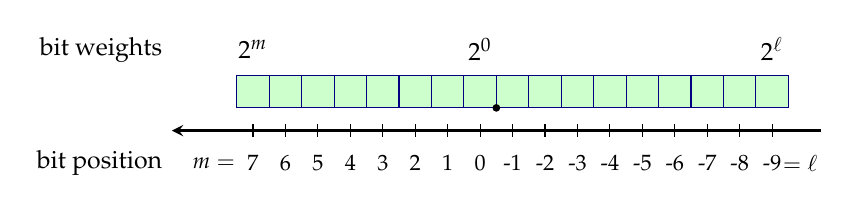
\begin{tikzpicture}[x=2.5ex, y=2.5ex]
        \fixpointnumber{0}{7}{-9}{0}
        \fixpointpositions{0}{7}{-9}{0}
        \fixpointweightsml{0}{7}{-9}{0}
      \end{tikzpicture}
  \end{center}
    \vspace{-2ex}
  \caption{An unsigned fix-point format $\UFix(m,\ell)$.}
  \label{fig:ufixformat}
\end{figure}


A fixed-point format may be signed or unsigned (\fig{fig:ufixformat}).
For signed formats the sign bit is at the position $m$.

\begin{figure}[h!]
  \begin{center}
     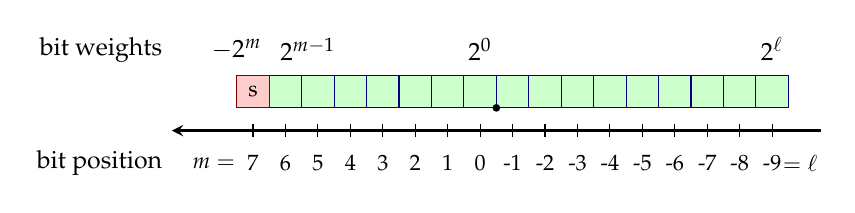
\begin{tikzpicture}[x=2.5ex, y=2.5ex]
        \fixpointnumber{1}{7}{-9}{0}
        \fixpointpositions{1}{7}{-9}{0}
        \fixpointweightsml{1}{7}{-9}{0}
      \end{tikzpicture}
    \end{center}
    \vspace{-2ex}
  \caption{A signed fixed-point format $\SFix(m,\ell)$.}
  \label{fig:sfixformat}
\end{figure}

For some operators, the signedness is a parameter. In this case it is a boolean  parameter (true for signed).

Now for a more stylistic, but nevertheless useful convention.
Whenever an interface (be it to the command line, or to an internal function) includes the MSB and the LSB of the same format, they should appear in this order (MSB then LSB).
This order corresponds to the order of the weights in the binary writing (the MSB is to the left of the LSB). 
When a boolean signedness is passed as well, it should be first, for the same reason (the sign bit is the leftmost bit).

Some examples of fixed-point formats:
\begin{itemize}
\item C char type corresponds to MSB=7, LSB=0.
\item a n-bit unsigned number between 0 and 1 has MSB=-1 and LSB=-n
\item a n-bit signed number between -1 and 1 has MSB=0 and LSB=-n+1
\end{itemize}

Finally, whenever we can live with integers, we should stick with integers and not obfuscate them as fixed-point numbers.



 

\subsubsection{Floating-point numbers}

FloPoCo partly supports two floating-point formats.

\paragraph{IEEE floating-point numbers}
The standard IEEE-754 is generalized to arbitrary exponent and mantissa sizes (see \fig{fig:ieee-fp-format})
 \begin{figure}[h]
   \centering
   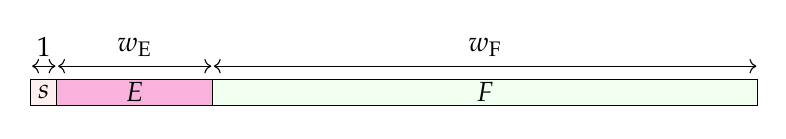
\begin{tikzpicture}
     \tikzset{x=1ex,y=1ex};
      \draw[fill=signbitfillcolor, fill opacity=0.3](0,0) rectangle ++(2,2) node[opacity=1,midway]{$s$};
      \draw[fill=magenta, fill opacity=0.3](2,0) rectangle ++(12,2) node[opacity=1,midway]{$E$};
      \draw[fill=normalbitfillcolor, fill opacity=0.3](14,0) rectangle ++(42,2) node[opacity=1,midway]{$F$};
      % the arrows
      \draw[<->,>=Computer Modern Rightarrow] (0.1,3) -- ++(1.8,0) node[midway,above] {$1$}; 
      \draw[<->,>=Computer Modern Rightarrow] (2.1,3) -- ++(11.8,0) node[midway,above] {$w_\text{E}$}; 
      \draw[<->,>=Computer Modern Rightarrow] (14.1,3) -- ++(41.8,0) node[midway,above] {$w_\text{F}$}; 
    \end{tikzpicture}
    \caption{Bit fields of an IEEE754-like  floating-point number of parameters $(\wE,\wF)$}
   \label{fig:ieee-fp-format}
 \end{figure}

 The exponent field is used to encode
 \begin{itemize}
 \item infinities (exponent field $E=11...11$, $F=0$),
 \item Not a Number or NaN (exponent field $E=11...11$, $F\ne 0$),
 \item subnormals (exponent field $E=00...00$, $F\ne 0$)
 \item (signed) zeroes (exponent field $E=00...00$, $F=0$)
 \end{itemize}

When not infinity and not NaN, the value of a floating-point vector may be defined as follows (where $E_0$ is  the \emph{exponent bias} and $n$ is the ``is normal'' bit):
\begin{eqnarray}
  E_0 &=& 2^{\wE-1}-1\\
 n &=&
\begin{cases}
0 \quad\text{ if } E=0 \\
1 \quad\text{ otherwise}
\end{cases}\nonumber\\
X &=& (-1)^{s}  \times 2^{E-E_0+1-n} \times (n+F) \quad .\label{eq:repr:normalbit}\nonumber
\end{eqnarray}

 
\paragraph{Simple floating-point numbers}

FloPoCo also supports a simpler format where  the exceptional cases (zero, infinity, NaN) are encoded in two additional bits (see \fig{fig:flopocoformat} and \tab{tab:formats:flopoco:exn}).
This makes it more hardware-efficient (no decoding/encoding of these exceptional cases in the exponent), but less memory-efficient.
Also, this format does not support subnormal numbers.

 \begin{figure}[h]
   \centering
   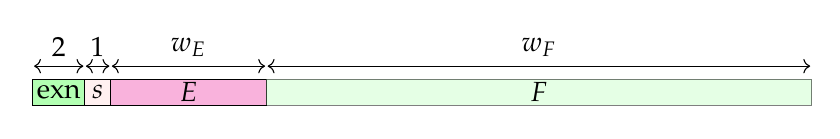
\begin{tikzpicture}
     \tikzset{x=1ex,y=1ex};
     % alternate bits, mac-like
      % \foreach \x in {0,...,14} { 
      %   \draw[line width=0,color=white,fill=normalbitfillcolor!25] ($(4*\x ex, 0)$)   rectangle  ++(2,2) ;
      %   \draw[line width=0,color=white,fill=normalbitfillcolor!50] ($(4*\x ex + 2ex, 0)$)   rectangle  ++(2,2) ;
      %   }
      \draw[fill=green, fill opacity=0.3](0,0) rectangle ++(4,2) node[opacity=1,midway]{exn};
      \draw[fill=signbitfillcolor, fill opacity=0.3](4,0) rectangle ++(2,2) node[opacity=1,midway]{$s$};
      \draw[fill=magenta, fill opacity=0.3](6,0) rectangle ++(12,2) node[opacity=1,midway]{$E$};
      \draw[fill=normalbitfillcolor, opacity=0.5](18,0) rectangle ++(42,2) node[opacity=1,midway]{$F$};
      % the arrows
      \draw[<->,>=Computer Modern Rightarrow] (4.1,3) -- ++(1.8,0) node[midway,above] {$1$}; 
      \draw[<->,>=Computer Modern Rightarrow] (0.1,3) -- ++(3.8,0) node[midway,above] {$2$}; 
      \draw[<->,>=Computer Modern Rightarrow] (6.1,3) -- ++(11.8,0) node[midway,above] {$\wE$}; 
      \draw[<->,>=Computer Modern Rightarrow] (18.1,3) -- ++(41.8,0) node[midway,above] {$\wF$}; 
   \end{tikzpicture}
   \caption{Bit fields of a flopoco  floating-point number of parameters $(\wE,\wF)$}
   \label{fig:flopocoformat}
 \end{figure}

When exn$=01$ (normal numbers), the value encoded is 
\begin{align}
  X = (-1)^{s} \times (1+{F}) \times 2^{E-E_0}\quad 
\end{align}
where $E_0$ is the same {exponent bias} as in IEEE-754  formats: $E_0 = 2^{\wE-1}-1$.

 \begin{table}[h]
  \centering
   \caption{Encoding of exceptional cases in the FloPoCo floating-point format}
   \label{tab:formats:flopoco:exn}
     \begin{tabular}{rl}
       \toprule
       exn &   meaning \\
       \midrule
       00 & zero (there are two zeroes, noted $+0$ and $-0$, according to $s$)\\
       01 & normal numbers \\
       10 & infinity ($+\infty$ or $-\infty$, according to $s$)\\
       11 &  NaN (Not a Number)\\
       \bottomrule
     \end{tabular}
 \end{table}

\paragraph{Brief comparison of the two formats}
Since the extremal values zero and infinity are not encoded as special exponent values, the exponent range for normal numbers is slightly larger than in the IEEE754 for the same value of $\wE$, as  \tab{tab:ieee-versus-flopoco-formats} shows.
%(also compare \fig{fig:flopocofloat32} and \fig{fig:nr:IEEENormals}). 
However a number in the FloPoCo format two more bits than a number in the IEEE754 format, for the same $(\wE,\wF)$.

\begin{table}[h!]
  \begin{center}
    \caption{Comparison of properties of the IEEE and FloPoCo formats. \label{tab:ieee-versus-flopoco-formats}}
    \begin{tabular}{C{2cm}C{5cm}C{4cm}}
      \toprule
                 & \IEEEFloat$(w_\text{E},w_\text{F})$                    &  \Float$(w_\text{E},w_\text{F})$                \\
      \midrule                                                                                
      bias value & \multicolumn{2}{c}{$E_0 = 2^{\wE-1}-1$}                                     \\ 
      \midrule                                                                                
      Total size & $w_\text{E}+w_\text{F}+1$ bits                         & $w_\text{E}+w_\text{F}+3$ bits                  \\
      $\emin$    & $ -2^{\wE-1}+2$                                        & $-2^{\wE-1}+1$                    \\
      $\emax$    & $2^{\wE-1}-1$                                          & $2^{\wE-1}$                       \\
      Smallest   & $2^{\emin-w_\text{F}}\ =\ 2^{-2^{\wE-1}+2-w_\text{F}}$ & $2^{\emin}\ =\ 2^{-2^{\wE-1}+1}$      \\
      Largest    & $(2-2^{-w_\text{F}})\cdot 2^{\emax}$                   & $(2-2^{-w_\text{F}})\cdot 2^{\emax}$      \\
      \bottomrule
    \end{tabular}       
  \end{center}
\end{table}

\subsubsection{Format conversion utilities for debugging} 
FloPoCo includes small useful programs that convert the binary string of a floating-point number to human-readable decimal, and back:
\begin{itemize}
\item \texttt{fp2bin} and \texttt{bin2fp} for the FloPoCo format;
\item \texttt{fp2ieee} and \texttt{ieee2fp} for the IEEE format.
\end{itemize}
\texttt{fp2bin}



\subsection{More on parameters}
All the parameters are provided to FloPoCo as \emph{name=value} pairs.

Each operator is heavily parameterized with functional and performance parameters.
To know the parameters of a given operator, just invoke flopoco for this operator without parameters, \eg, \mbox{\texttt{flopoco FPAdd}}. 

\begin{figure}[]
  \small
  \centering
  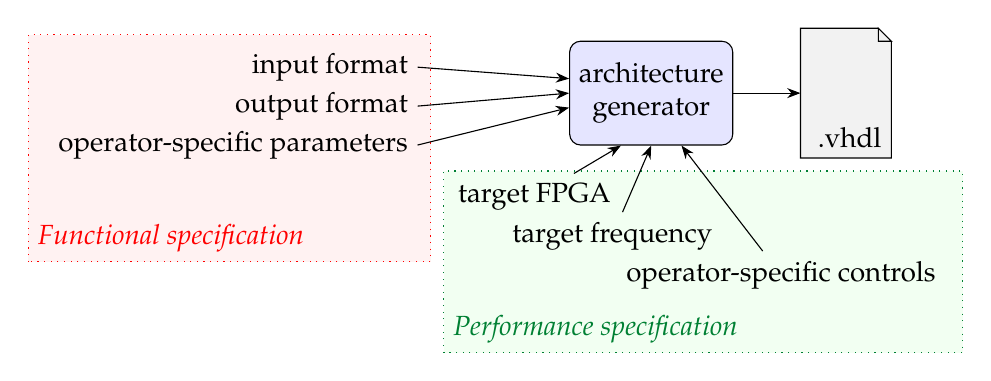
\begin{tikzpicture}[x=1ex,y=1ex]
    \draw(-48,-11) coordinate(fsbl);
    \draw[dotted,red,fill=red!5] (fsbl) rectangle +(31,17.5);   
    \draw(fsbl)  node[above right,red] {\emph{Functional specification}};   
%    \draw(fsbl)  node[above right,red!90] {\emph{\emph{Functional specification}};   
    \draw(-16,-18) coordinate(psbl);
    \draw[dotted,darkgreen,fill=green!5] (psbl) rectangle +(40,14);   
    \draw(psbl)  node[above right,darkgreen] {\emph{Performance specification}};   
    \node[draw,align=center,fill=blue!10,rounded corners, minimum width=12ex, minimum height=8ex] (flopoco) at (0,2) {architecture\\generator};
    \node[left] (ai)      at (-18,4)  {input format};   
    \node[left] (precx)   at (-18,1) {output format};   
    \node[left] (precy)   at (-18,-2) {operator-specific parameters};   
    \node[] (degree)  at (-9,-6) {target FPGA};   
    \node[] (target)  at (-3,-9) {target frequency};   
    \node[] (freq)    at (10,-12)  {operator-specific controls};   
    \vhdlfile{15ex}{2ex};
    \draw[->,>=Stealth] (ai.east) -- (flopoco.170) ;
    \draw[->,>=Stealth] (precx.east) -- (flopoco.180) ;
    \draw[->,>=Stealth] (precy.east) -- (flopoco.190) ;
    \draw[->,>=Stealth] (degree) -- (flopoco.240) ;
    \draw[->,>=Stealth] (target) -- (flopoco.270) ;
    \draw[->,>=Stealth] (freq) -- (flopoco.300) ;
    \draw[->,>=Stealth] (flopoco.east) -- (vhdl.west) ;
  \end{tikzpicture}
  \caption[]{Interface to a flopoco Operator}
  \label{fig:flopoco:genericinterface}
\end{figure}


As illustrated in   \fig{fig:flopoco:genericinterface}, parameters can be broadly separated in two classes: \emph{functional} parameters specify the function, while \emph{performance} parameters control the performance and its many trade-offs (such as memory versus compute, area versus speed, frequency versus latency, etc.).

A general rule is that functional parameters should be mandatory with no default value, while performance parameters should be optional with a sensible default value.
However, there are exceptions to both rules.
For instance, there is one parameter to \texttt{FPAdd} which decides if the operator should be an adder or a subtracter.
This is a functional parameter, but its default is set to addition, because we feel it is the most common case.
Conversely, \texttt{FixFunctionByPiecewisePoly} has a mandatory parameter for the degree to be used, although it is definitely a performance parameter.
The reason here is that we feel that the decision of a ``sensible default value'' is too application-dependent.

For a given operator, there are usually many parameter combinations that do not make sense.
We attempt to filter them and provide sensible error messages in such cases, but users often have more imagination that developers can anticipate, and invalid combinations of parameter values may lead to unexpected crashes or non-working VHDL.


\subsection{Global options}
Several global options are available.
They are also specified as  \emph{name=value} pairs and will typically change the operators occuring after them in the list. 
Here is a non-exhaustive list, the full list is available on the command line when typing \texttt{flopoco} with no argument.

\begin{itemize}
\item \texttt{target=Virtex5}  sets the target hardware family.
  	For a list of supported families see the command line. 
	We typically target the highest speed grade available for a family.
\item \texttt{frequency=300} sets the target frequency (in MHz). FloPoCo will attempt to pipeline the operator for this frequency (see \sect{sec:flopoco:pipelining:user} below).
\item \texttt{name=UserProvidedName} replaces the (ugly and parameter-dependent) entity name generated by FloPoCo for the next operator. 
This allows in particular to change parameters while keeping the same entity name, so that these changes are transparent to the rest of the project.
\item \texttt{plainVHDL=yes} instructs FloPoCo to output concise and readable VHDL, using only + and * VHDL operators instead of FloPoCo adders and multipliers.
This helps understanding the algorithms used by FloPoCo, but typically prevents or degrades automatic pipelining. 
\item \texttt{useHardMult=no} instructs FloPoCo not to use hard multipliers or DSP block.
\item \texttt{hardMultThreshold=0.7} instructs FloPoCo to use a hard multiplier (or DSP block) if less than 70\% of this hard multiplier are unused. 
 The ratio is between 0 and 1, such that
 0 means: any sub-multiplier that does not fully fill a DSP goes to logic; 
 1 means: any sub-multiplier, even very small ones, will consume a DSP.
\item \texttt{generateFigures=1}, for some operators, will generate relevant graphics in SVG or LaTeX.
\item \texttt{dependencyGraph=<no|compact|full>}  generates data dependency graphs. 
\item \texttt{clockEnable=false}, FloPoCo will add clock enable signals for every pipeline stage. 
\item \texttt{nameSignalByCycle=false}, when true then the delayed signals are named by their cycle instead of their delay. This is automatically set to true when clock enable is true. 

\end{itemize}


\subsection{Do not trust FloPoCo, the test bench is included}

FloPoCo is able to generate an infinite number of different operators, and the developers have obviously not tested each of them.
This issue is intrinsic to application-specific arithmetic.
A simple solution developed in FloPoCo is that  each operator comes with a test bench generator that will exercise exactly the operator being generated.

Details about the construction of these test benches can be found in the developer manual (see \url{http://flopoco.org/} for the latest version).
The point  to stress here is that the resulting test benches can be trusted by users.
The main reason for this is that the test vectors are not built out of the VHDL being generated, but out of the mathematical specification of the operator (as a mathematical function combined with a well-defined rounding, implemented in C++, see \sect{sec:test-bench-gener} below).
Thus, the probability of a bug in the VHDL being hidden by a bug in the test bench is very low.
In addition,  the code that generates testbenches is very small, quite boilerplate, and based on reference multiple-precision libraries that are well specified and well established: {GMP} and {MPFR}.
For this reason, the confidence in the test bench is much higher than the confidence in the generated VHDL.

The test bench generation also provides how the open-source VHDL simulator nvc (\url{https://github.com/nickg/nvc}) can be invoked to test the circuit. 
We highly recommend this fast and reliable command line simulator.
The command line is sufficient as it tells the user/developer if everything went fine (\texttt{0 error(s) encoutered}) or the test cases that failed.
In this case, waveform are written by nvc and calls to the open-source waveform viewer gtkwave (\url{https://gtkwave.sourceforge.net}) are provided that allows to further debug what went wrong.

The user interface to the test bench generation is kept extremely simple, to encourage users to test their FloPoCo operators.

\begin{flopocobox}{TestBench generation in FloPoCo}
  The following command builds a divider by 3 for 16-bit integers, and an exhaustive test bench for this operator:
 
  \flopoco{flopoco IntConstDiv wIn=16 d=3  TestBench } 

  This command creates a VHDL file and a (human-readable) \texttt{test.input} file containing all the possible values of the input and the corresponding expected output.
  It also outputs instructions to launch this test using a choice of VHDL simulators.
\end{flopocobox}

\begin{flopocobox}{Operation-specific testBench generation}
  For operators having a large input word size, exhaustive testing is out of reach.
  In such cases, the test should be limited to a smaller number of test vectors.
  The following command is an example of a (\Float) binary32 floating-point adder with 100,000 random tests.

  \flopoco{flopoco FPAdd we=8 wf=23 TestBench n=100000}  
  This testbench actually begins with all the corner-case test vectors that the developers of \texttt{FPAdd} could think of, including a few regression test vectors corresponding to past bugs.

  In addition, the random number generator used there is specific to the operator under test: with two random bit strings as inputs, the probability of a cancellation in the addition would be quite low, since it only happens when the exponents differ at most by 1.
  To  properly test this important feature of floating-point addition, the random generator  used has been slightly tweaked to make cancellations more frequent.
  See the developer manual for more details.
\end{flopocobox}
  



\subsection{Obscure branches and code attics}
The installation instructions on the web site currently use  the \texttt{master} branch of the Git repository of FloPoCo.
Beyond this branch, there are quite a few other, more experimental branches and forks where one may find rarer operators, or code snapshots that ensure that a publication is reproducible.

In principle, developers are encouraged to merge  their work in the master branch as soon as it may be of general use.
They are also encouraged  to clean up the master branch of experimental code, over-parameterization for research purpose, or obsolete variants for which a better option is available.
Unfortunately, they often do not have the time for these two time-consuming tasks, and we do apologize for this.
Any feedback on what should be prioritized will be welcome.

Quite often, a change to the FloPoCo framework (or to one of the libraries it uses) breaks some operators.
If these operators are not fixed by their original developers, the maintainers end up disabling them in the master branch.
Usually the code is just unplugged, not removed, : it is kept in ``attic'' directories or ``obscure branches'', where it may still compile, or not.
In any case, this code is still there for review and/or porting to the current framework, should the need arise.
Examples of code which is currently disabled but would deserve to be revived include the HOTBM function approximator by Jérémie Detrey \cite{DetDin2005:asap}, the LNS operators by Caroline Collange \cite{VouzisCollangeArnold2010}, the FPGA-specific random number generators by David Thomas \cite{thomas-13-table-hadamard-grng}, among many others.



%A the time of writing this book, examples of code only present in Obscure Branches include , 



\subsection{Automatic pipelining, the user point of view\label{sec:flopoco:pipelining:user}}

Most operators presented in this book are combinatorial circuits: they have no memory, the result only depends of the input, not of the past history of the operator. 
This is another direct consequence of the definition of an operator as the composition of a mathematical function\footnote{The main exceptions are the floating-point accumulators and the filters. There could be some day iterative variants of dividers, CORDIC operators, and in general digit-recurrence algorithms, but none of these is currently available in FloPoCo: the tool provides only the unrolled, combinatorial variants.} and a well-defined rounding.


\begin{figure}
  \centering
  \newcommand{\pipeN}{3}
  \subfigure[A combinatorial operator, with registers that produce its inputs and consume its outputs \label{fig:flopoco:genericpipe1} ]{
    \scalebox{.9}{
      \begin{tikzpicture}[x=1ex, y=1ex]        
        \draw (8*1.5,0) node[hwblock, fill=black!10, minimum width=32ex,minimum height=6ex] {} ;
        \foreach \x in {0,1,...,\pipeN} {
          \draw (8*\x,0) node[hwblock, minimum width=4ex,minimum height=4ex] (n\x)  {} ;
        }
        \draw (n\pipeN) ++ (8,0)  node[hwregblock] (regout) {};
        \drawclockinput{regout};
        \draw (n0) ++(-8,0) node[hwregblock] (regin) {};
        \drawclockinput{regin};
        
        \foreach \x/\y in {0/1,1/2,2/3} {
          \draw[hwbus,->] (n\x) -- (n\y) ;
        }
        \draw[hwbus,->] (n3) -- (regout) ;
        
        % \draw (0,0) node[hwblock, minimum width=30ex,minimum height=4ex] (n0)  {} ;
        \draw[hwbus,<-] (regin) -- ++(-3,0);
        \draw[hwbus,->] (regin) -- (n0) node[pos=.3, below]{$X$};
        \draw[hwbus,->] (regout) -- ++(3,0) node[below]{$Y$};
        
        \draw(regin.north) ++(0,1.2) coordinate(a); 
        \draw(regout.north) ++(0,1.2) coordinate(b); 
        \draw[ultra thick, red, ->] (a) -- (b) node[midway, above] {$\overline{\Delta t}$}; 

        \begin{scope}[xshift=-19ex, yshift=-20ex,y=2.5ex]          
          \pgfmathsetmacro{\period}{20} 
          \pgfmathsetmacro{\risex}{.5} % the slope lasts .3
          \pgfmathsetmacro{\phase}{0.5*\period} 
          \draw[->] (-3,0) -- ++(65,0) node[right]{$t$};
          \draw[<->] (0,-.4) -- ++(\period,0) node[midway, below] {$\overline{\Delta t}$}; 

          % x=0 is the first clock rising edge
          \draw[blue,thick] (-1,.8) node[black,above left] {clk} --  ++(1,0) -- ++(0,1) coordinate(tmp);
          \foreach \x in {0,1,...,2} {
            \draw[dotted] (tmp)  ++(0,-2)  -- ++(0, 6);
            \draw[blue,thick] (tmp)--  ++(\phase,0) -- ++ (0,-1) -- ++(\phase,0)-- ++ (0,1) coordinate(tmp);
          }
          \draw[dotted] (tmp)  ++(0,-2)  -- ++(0, 6);

          % X
          \draw[green!37!black,thick] (-1,4) node[black,above left] {$X$} -- ++(1,0)  coordinate(tmp) ++(0,1) -- ++(-1,0) ;
          \foreach \i in {0,...,2} {
            \draw[green!37!black,thick] (tmp) -- ++(\risex,1) --  ++(\period-\risex,0) ++(0,-1) coordinate(tmp) -- ++(-\period+\risex,0) -- ++(-\risex,1) ++ (0.5*\period, -.55) node{$X_\i$};
          }
          % Y
          \draw[green!37!black,thick] (-1,2.5) node[black,above left] {$Y$} -- ++(1,0)  coordinate(tmp) ++(0,1) -- ++(-1,0) ;
          \foreach \i in {0} {
            \draw[green!37!black,thick] (tmp) -- ++(\risex,1) --  ++(\period-\risex,0) ++(0,-1) coordinate(tmp) -- ++(-\period+\risex,0) -- ++(-\risex,1);
          }
          \foreach \i in {0,1} {
            \draw[green!37!black,thick] (tmp) -- ++(\risex,1) --  ++(\period-\risex,0) ++(0,-1) coordinate(tmp) -- ++(-\period+\risex,0) -- ++(-\risex,1) ++ (0.5*\period, -.55) node{$Y_\i$};
          }          
        \end{scope}
      \end{tikzpicture}
    }
  }
  
 
  \subfigure[The same operator, pipelined into $N=4$ stages: frequency can be multiplied by 4.\label{fig:flopoco:genericpipe2}]{
    \scalebox{.9}{
      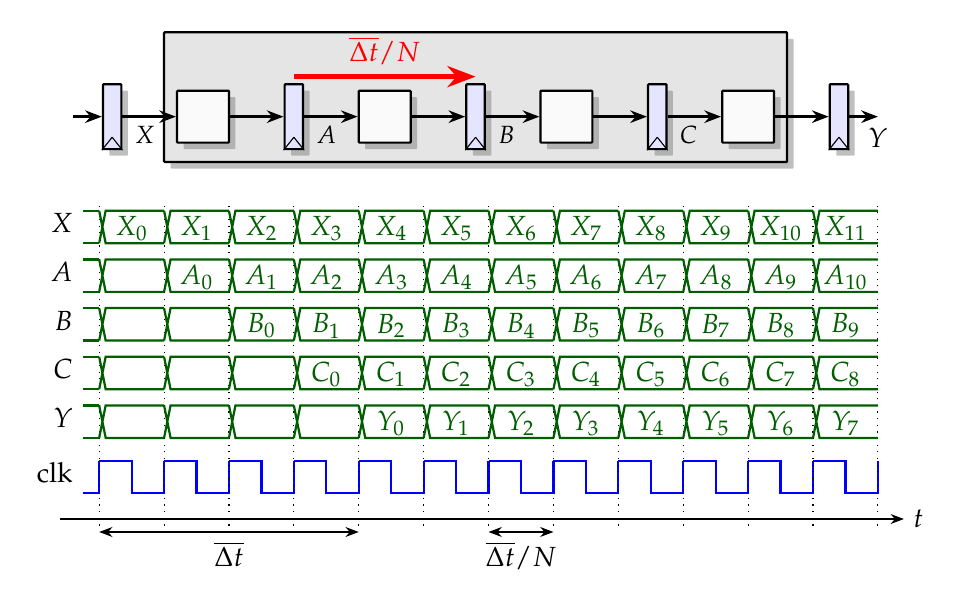
\begin{tikzpicture}[x=1ex, y=1ex]
        \draw (21,1.5) node[hwblock, fill=black!10, minimum width=48ex,minimum height=10ex] {} ;
        \foreach \x in {0,1,2,3} {
          \draw (14*\x,0) node[hwblock, minimum width=4ex,minimum height=4ex] (n\x)  {} ;
        }
        \foreach \x in {0,1,2,3} {
          \draw (n\x) ++(7,0) node[hwregblock](r\x)  {} ;
          \drawclockinput{r\x};
          \draw[hwbus,->] (n\x) -- (r\x)  {};
        }
        \draw (n0) ++(-7,0) node[hwregblock](rin)  {} ;
        \drawclockinput{rin};
        \foreach \x/\y/\i in {rin/n0/X,r0/n1/A, r1/n2/B, r2/n3/C} {
          \draw[hwbus,->] (\x) -- (\y);
          \draw (\x) ++(1,-1.4) node[right]{\small$\i$};
        }
        \draw[hwbus,<-] (rin) -- ++(-3,0);
        \draw[hwbus,->] (r3) -- ++(3,0) node[below]{$Y$};
        \draw(r0.north) ++(0,.5) coordinate(a); 
        \draw(r1.north) ++(0,.5) coordinate(b); 
        \draw[ultra thick, red, ->] (a) -- (b) node[midway, above] {$\overline{\Delta t}/N$}; 

        \begin{scope}[xshift=-8ex, yshift=-31ex,y=2.5ex]
          \pgfmathsetmacro{\period}{5} 
          \pgfmathsetmacro{\risex}{.5} % the slope lasts .3
          \pgfmathsetmacro{\phase}{0.5*\period} 
          \draw[->] (-3,0) -- ++(65,0) node[right]{$t$};
          \draw[<->] (6*\period,-.4) -- ++(\period,0) node[midway, below] {$\overline{\Delta t}/N$}; 
          \draw[<->] (0,-.4) -- ++(4*\period,0) node[midway, below] {$\overline{\Delta t}$}; 
          % x=0 is the first clock rising edge
          \draw[blue,thick] (-0.5*\phase,.8) node[black,above left] {clk} --  ++(0.5*\phase,0) -- ++(0,1) coordinate(tmp);
          \foreach \x in {0,1,...,11} {
            \draw[dotted] (tmp)  ++(0,-2)  -- ++(0, 10);
            \draw[blue,thick] (tmp)--  ++(\phase,0) -- ++ (0,-1) -- ++(\phase,0)-- ++ (0,1) coordinate(tmp);
          }
          \draw[dotted] (tmp)  ++(0,-2)  -- ++(0, 10);

          % X
          \draw[green!37!black,thick] (-0.5*\phase,8.5) node[black,above left] {$X$} -- ++(0.5*\phase,0)  coordinate(tmp) ++(0,1) -- ++(-0.5*\phase,0) ;
          \foreach \i in {0,1,...,11} {
            \draw[green!37!black,thick] (tmp) -- ++(\risex,1) --  ++(\period-\risex,0) ++(0,-1) coordinate(tmp) -- ++(-\period+\risex,0) -- ++(-\risex,1) ++ (0.5*\period, -.55) node{$X_{\i}$};
          }

          % A
          \draw[green!37!black,thick] (-0.5*\phase,7) node[black,above left] {$A$} -- ++(0.5*\phase,0)  coordinate(tmp) ++(0,1) -- ++(-0.5*\phase,0) ;
          \foreach \i in {0} {
            \draw[green!37!black,thick] (tmp) -- ++(\risex,1) --  ++(\period-\risex,0) ++(0,-1) coordinate(tmp) -- ++(-\period+\risex,0) -- ++(-\risex,1);
          }
          \foreach \i in {0,...,10} {
            \draw[green!37!black,thick] (tmp) -- ++(\risex,1) --  ++(\period-\risex,0) ++(0,-1) coordinate(tmp) -- ++(-\period+\risex,0) -- ++(-\risex,1) ++ (0.5*\period, -.55) node{$A_{\i}$};
          }

          % B
          \draw[green!37!black,thick] (-0.5*\phase,5.5) node[black,above left] {$B$} -- ++(0.5*\phase,0)  coordinate(tmp) ++(0,1) -- ++(-0.5*\phase,0) ;
          \foreach \i in {0,1} {
            \draw[green!37!black,thick] (tmp) -- ++(\risex,1) --  ++(\period-\risex,0) ++(0,-1) coordinate(tmp) -- ++(-\period+\risex,0) -- ++(-\risex,1);
          }
          \foreach \i in {0,...,9} {
            \draw[green!37!black,thick] (tmp) -- ++(\risex,1) --  ++(\period-\risex,0) ++(0,-1) coordinate(tmp) -- ++(-\period+\risex,0) -- ++(-\risex,1) ++ (0.5*\period, -.55) node{$B_{\i}$};
          }

          % C
          \draw[green!37!black,thick] (-0.5*\phase,4) node[black,above left] {$C$} -- ++(0.5*\phase,0)  coordinate(tmp) ++(0,1) -- ++(-0.5*\phase,0) ;
          \foreach \i in {0,1,2} {
            \draw[green!37!black,thick] (tmp) -- ++(\risex,1) --  ++(\period-\risex,0) ++(0,-1) coordinate(tmp) -- ++(-\period+\risex,0) -- ++(-\risex,1);
          }
          \foreach \i in {0,...,8} {
            \draw[green!37!black,thick] (tmp) -- ++(\risex,1) --  ++(\period-\risex,0) ++(0,-1) coordinate(tmp) -- ++(-\period+\risex,0) -- ++(-\risex,1) ++ (0.5*\period, -.55) node{$C_{\i}$};
          }
          % Y
          \draw[green!37!black,thick] (-0.5*\phase,2.5) node[black,above left] {$Y$} -- ++(0.5*\phase,0)  coordinate(tmp) ++(0,1) -- ++(-0.5*\phase,0) ;
          \foreach \i in {0,1,2,3} {
            \draw[green!37!black,thick] (tmp) -- ++(\risex,1) --  ++(\period-\risex,0) ++(0,-1) coordinate(tmp) -- ++(-\period+\risex,0) -- ++(-\risex,1);
          }
          \foreach \i in {0,...,7} {
            \draw[green!37!black,thick] (tmp) -- ++(\risex,1) --  ++(\period-\risex,0) ++(0,-1) coordinate(tmp) -- ++(-\period+\risex,0) -- ++(-\risex,1) ++ (0.5*\period, -.55) node{$Y_{\i}$};
          }          
        \end{scope}
      \end{tikzpicture}
    }
  }
  \caption{Pipelining a combinatorial operator}
  \label{fig:flopoco:genericpipe}
\end{figure}

Another point of view is that the directed graph of subcomponents that describes the circuit (down to the gates or whatever elementary processing elements of the technology) is acyclic.
However, each component of this graph needs some time (and some energy) to perform its computation.
If an input is presented at time $t_0$, the correct output will be computed after some delay $\Delta t$ (measured in seconds).
This delay may depend on the input.
Its maximum value over all the possible inputs is called the \emph{critical path delay} of the circuit, noted $\overline{\Delta t}$.
If the operator is sandwiched between input registers and output registers as illustrated by \fig{fig:flopoco:genericpipe1}, then the input registers may present a new input every $\overline{\Delta t}$ period, and the circuit will have the time to process this input (and register the result in the output registers) before the next input is presented.
In other words, the operator can operate at frequency $1/\overline{\Delta t}$.

Pipelining is a technique that allows an operator to function at a higher frequency by dividing the circuit graph into $N$ slices called \emph{pipeline stages}, determined such that the critical path delay of each slice is about $\overline{\Delta t}/N$.
Registers are inserted between slices to hold intermediate computations, as illustrated by \fig{fig:flopoco:genericpipe2}.
If the pipeline is ideally balanced, and ignoring the delay added by these extra registers, the frequency can become $N/\overline{\Delta t}$: compared to the combinatorial circuit, the frequency has been multiplied by $N$.
The cost is additional registers.
In practice, however, it is difficult to achieve a perfectly balanced pipeline, and the registers add some delay which limits the achievable frequency \cite{Hri2002,Sprangle2002}.

Pipelining combinatorial operators is simple in theory but time-consuming if performed by hand.
As \fig{fig:flopoco-fpadd-pipe} illustrates, actual operators are often more complex than \fig{fig:flopoco:genericpipe}.
FloPoCo therefore automates this task.
The interface for it is simply the target frequency provided through the \texttt{frequency} parameter.
An important remark on \fig{fig:flopoco-fpadd-pipe} is that FloPoCo does not add any input and output registers.
All it does is insert the intermediate (pipeline) registers.
The ``pipeline depth'' it reports is the number of synchronization barriers inserted (this information is also provided in comments before each entity declaration in the generated VHDL).

The resulting pipeline is quite good for practical purposes.
Note however that FloPoCo  does not pretend to generate an optimal pipeline (an optimal pipeline would minimize the overall cost of the registers while achieving a given target frequency  \cite{LeisersonSaxe1991}).
It does not even guarantee that the operator will operate at the prescribed frequency -- we are at the mercy of the backend tools that will transform the VHDL into an actual circuit.
Indeed,  these tools are the proper place for fine-tuning a pipeline.
However, it does guarantee that the pipeline is well synchronized (and \texttt{TestBench} adapts to pipelined operators for users to check).
Hence, cases where the required frequency is not reached or even too high can be easily fixed by adjusting the target frequency accordingly.
Note that this may be done on a per-operator basis, as in:\\
		 \texttt{flopoco  FPAdd frequency=200 wE=11 wF=53 FPMult frequency=300 wE=8 wF=23}



\begin{flopocobox}{Sandwiching an operator with register}
  In order to measure the actual operating frequency at which an operator runs, it is important to add the registers on the inputs and outputs.
  FloPoCo provides an operator that sandwiches between registers the operator preceding it on the command line (just like \texttt{TestBench} tests the preceding operator).

  \flopoco{flopoco frequency=400 FPAdd wE=8 wF=23   RegisterSandwich} 
\end{flopocobox}





\newcommand{\fpadd}{
      \draw (0,7) node[hwblock, minimum height=4ex, minimum width=40ex] (unpack) {unpack \& exception handling, \\exponent difference \& swap};
      \draw[hwwire,<-] (unpack.170)  -- ++(0,3) node[above]{$\text{add}/\overline{\text{sub}}$}  coordinate[pos=0.7] (bw);
      \draw[hwbus,<-] (unpack.30)  -- ++(0,3) node[above]{$Y_\text{in}$}  coordinate[pos=0.7] (bw);
      \draw[hwbus,<-] (unpack.150) -- ++(0,3) node[above]{$X_\text{in}$}  coordinate[pos=0.7] (bw);

      \draw(unpack.south) ++(-4,0) coordinate(xout);
      \draw[hwbus] (xout) -- ++(0,-1.7) node[left]{};
      
      \draw(unpack.south) ++(4,0) coordinate(yout);
      \draw (yout) ++ (0,-7) node[hwblock, minimum height=6ex, minimum width=8ex] (shifter) {\Large $>>$};
      \draw[hwbus, ->] (yout) -- ++(0,-1.7) node[left]{} --  (shifter.north) coordinate[pos=0.1](bw) ;
      %\bitwidth{bw}{$w_F+1$}{r};
      \draw[hwbus, ->] (unpack.350) -- ++(0,-1.7)	 node[right]{}  |-  (shifter.east)   node[pos=0.4](bw){};
      %\bitwidth{bw}{$\ceil{\log_2(w_F+2)}$}{r};
      \draw (unpack.south) ++ (0,-17) node[hwblock, minimum height=6ex, minimum width=14ex] (add) { $|M_x\pm M_{Y_\text{a}}|$};
      \draw (add.west) ++(-16,-4)  node(xor) [xor gate, point down,circuit symbol unit=4pt]{};
      
      \draw[hwbus, ->] (shifter.south) -- ++(0,-4) coordinate[pos=0.4](reg1) node[pos=0.4](bw){} node[midway, left]{};
      %\bitwidth{bw}{$w_F+3$}{r};
      \draw[hwbus, ->] (xout) -- ++(0,-14) coordinate[pos=0.82](reg2) node[pos=0.4](bw){};

      \draw (add.south) ++ (0,-7) node[hwblock, minimum height=6ex] (lzcshifter) { LZC\\+ shifter};
      \draw (lzcshifter.south) ++ (-2,-7) node[hwblock, minimum height=5ex, minimum width=18ex] (round) {rounding  adder};
      \draw (lzcshifter.south west) ++ (-9,-1) node[hwblock, minimum height=3ex, minimum width=7ex] (expupdate) {\Large$-$};

      \draw[hwbus]  (expupdate.140) ++(0,6)  node[hwblock, minimum height=2ex, minimum width=6ex](expinc) {$+1$};

      \draw ($(unpack.260)!(expinc.south)!(unpack.280)$) coordinate(exout);
      \draw[hwbus] (exout) -- ++(0,-1.7) node[left]{} ++ (0,-2)  coordinate[](bw);
      %\bitwidth{bw}{$w_E$}{r};

      \draw[hwbus, ->] (exout) --  (expinc)  coordinate[pos=0.53](reg3) coordinate[pos=0.72](reg4);
      \draw[hwbus, ->]  (expinc) -- (expupdate.140) coordinate[pos=0.38](reg11) coordinate[midway](bw);
      %\bitwidth{bw}{$w_E+1$}{l};
      \draw[hwbus, ->] (lzcshifter.west) -| (expupdate.40) coordinate[pos=0.25](reg9) node[pos=0.45, above] {};
      \draw[hwbus, ->] (expupdate.south) |- (round.175) coordinate[pos=0.3](bw);
      %\bitwidth{bw}{$w_E+2$}{l};
      \draw[hwbus, ->] (add.south) -- (lzcshifter.north) coordinate[pos=0.5](reg8) node[midway, left]{};
      %\bitwidth{bw}{$w_F+4$}{r};
      \draw[hwbus, ->] (lzcshifter.south) -- ($(round.80)!(lzcshifter.south)!(round.100)$) coordinate[pos=0.5](bw) coordinate[pos=0.4](reg13) node[midway, left]{};
      %\bitwidth{bw}{$w_F+1$}{r};
      \draw (round.south) ++(0,-6)  node[hwblock, minimum height=4ex, minimum width=30ex] (finalexn) {exception handling \& pack};
      \draw[hwbus, ->] (round.south) -- (finalexn.north) coordinate[pos=0.4](bw) ;
      %\bitwidth{bw}{$w_E+2+w_F$}{l};
      \draw[hwwire, ->] (lzcshifter.east) -- ++(1,0) node[above right]{} -| (finalexn.10)coordinate[pos=0.65](reg12);

      \draw[hwwire, ->] (xor.output) |- (finalexn.west) coordinate[pos=0.09](reg10) node[pos=0.5, left] {} ;
      \draw[hwbus, ->] (unpack.east) -- ++(2,0) node[pos=0.6, above, font=\small]{} |- (finalexn.east) coordinate[pos=0.15](reg14) coordinate[pos=0.26](reg15) coordinate[pos=0.36](reg16) coordinate[pos=0.5](bw) ;

      \draw[hwwire, ->] (unpack.west) -- ++(-3,0) coordinate (sx) node[above] {};
      \draw[hwwire] (sx) -| (xor.input 2) coordinate[pos=0.83] (reg5)  coordinate[pos=0.92] (reg6)  ;
      \draw(unpack.south) ++(-12,0) coordinate(sy);
      \draw[hwwire,->] (sy) |- (add.170) coordinate[pos=0.365] (reg7) node[pos=0.3,right]{};
      \draw[white,line width=0.6ex] (add.190) ++(-3,0) --++(-6,0) ; 
      \draw[hwwire,->] (add.190) -- ++(-3,0); %;
      \draw[hwwire] (add.190)  -| (xor.input 1) node[pos=0.4,above]{}; 

      \draw[hwbus, ->] (finalexn.south) -- ++(0,-3)	 node[below]{$R$};

  }

  \begin{figure}[]
    \centering
    \subfigure[Adding 3 synchronization barriers -- FloPoCo reports a pipeline depth of 3 -- means that there are 4 pipeline stages  \label{fig:flopoco:fpaddpipe}]{
      \scalebox{0.8}{
        \begin{tikzpicture}[x=1ex,y=1ex,circuit logic US]
          \fpadd
          \draw[blue, dashed, ultra thick] (shifter.south) ++(-29, -1.9) -- ++(57,0)
          ++(0,3) node [above left, align=left]{pipeline\\stage 0}
          ++(0,-5) node [below left, align=left]{pipeline\\stage 1};
          
          \draw[blue, dashed, ultra thick] (add.south) ++(32, -2)   -- ++(-42,0)  -- ++(-4,6)     -- ++(-11,0) ;
          
          \draw[blue, dashed, ultra thick] (lzcshifter.south) ++(32, -2)  ++(0,1.5) node [above left, align=left]{pipeline\\stage 2}++(0,-1.5)  ++(0,-3) node [below left, align=left]{pipeline\\stage 3}++(0,3)  -- ++(-38,0)  -- ++(-4,5.5)     -- ++(-15,0)  ;
        \end{tikzpicture}
      }
    }
    \hfill
    \subfigure[The corresponding registers are inserted automatically by FloPoCo \label{fig:flopoco:fpaddpipereg}]{
      \scalebox{0.8}{
        \begin{tikzpicture}[x=1ex,y=1ex,circuit logic US]
          \fpadd
          \draw[blue, dashed, ultra thick] (shifter.south) ++(-29, -1.9) -- ++(49,0);
          
          \draw[blue, dashed, ultra thick] (add.south) ++(24, -2)   -- ++(-34,0)  -- ++(-4,6)     -- ++(-11,0) ;
          
          \draw[blue, dashed, ultra thick] (lzcshifter.south) ++(24, -2)    -- ++(-30,0)  -- ++(-4,5.5)     -- ++(-15,0)  ;
          \draw (reg1) node[hwregblock, minimum height=.5ex, minimum width=6ex] {};
          \draw (reg2) node[hwregblock, minimum height=.5ex, minimum width=6ex] {};
          \draw (reg3) node[hwregblock, minimum height=.5ex, minimum width=4ex] {};
          \draw (reg4) node[hwregblock, minimum height=.5ex, minimum width=4ex] {};
          \draw (reg5) node[hwregblock, minimum height=.5ex, minimum width=.5ex]{};
          \draw (reg6) node[hwregblock, minimum height=.5ex, minimum width=.5ex]{};
          \draw (reg7) node[hwregblock, minimum height=.5ex, minimum width=.5ex]{};
          \draw (reg8) node[hwregblock, minimum height=.5ex, minimum width=6ex] {};
          \draw (reg9) node[hwregblock, minimum height=.5ex, minimum width=4ex,rotate=90]{};
          \draw (reg10) node[hwregblock, minimum height=.5ex, minimum width=.5ex]{};
          \draw (reg11) node[hwregblock, minimum height=.5ex, minimum width=4ex] {};
          \draw (reg12) node[hwregblock, minimum height=.5ex, minimum width=.5ex]{};
          \draw (reg13) node[hwregblock, minimum height=.5ex, minimum width=4ex] {};
          \draw (reg14) node[hwregblock, minimum height=.5ex, minimum width=1ex] {};
          \draw (reg15) node[hwregblock, minimum height=.5ex, minimum width=1ex] {};
          \draw (reg16) node[hwregblock, minimum height=.5ex, minimum width=1ex] {} ;
          %\draw (reg2) node[hwregblock, minimum height=.5ex, minimum width=6ex]{};
%          \draw (reg2) node[hwregblock, minimum height=.5ex, minimum width=6ex]{};
%          \draw (reg2) node[hwregblock, minimum height=.5ex, minimum width=6ex]{};
        \end{tikzpicture}
      }
    }
    \caption{Pipelining a floating-point adder}
    \label{fig:flopoco-fpadd-pipe}
  \end{figure}












\subsection{Synthesis helper tools}
  FloPoCo also provides (in the \texttt{tools/} directory) small python scripts that will synthesize an operator for an FPGA using either Vivado or Quartus.
  These tools read in the VHDL file the target information, launch synthesis accordingly, and report the main synthesis result on the console.




\section{Tutorial for new developers \label{sec:tutorial}}

The FloPoCo distribution include a dummy tutorial operator in \texttt{src/TutorialOperator.hpp} and \texttt{src/TutorialOperator.cpp}.
It describes an operator class \texttt{TutorialOperator} that you may freely modify without disturbing the rest of FloPoCo.

\texttt{TutorialOperator} is heavily documented, and this section assumes that you are looking at it.

After compiling FloPoCo, run in a terminal\\
\verb!./flopoco TutorialOperator!

You will obtain the documentation on the parameters of this operator.
This documentation is defined by the \texttt{TutorialOperator::registerFactory} method.

Now run in a terminal\\
\verb!./flopoco TutorialOperator param0=8 param1=8!

and you should obtain  some VHDL in \texttt{flopoco.vhdl}

\subsection{Overview of FloPoCo code organization}

In the \texttt{code/} directory, there are several subdirectories:
\begin{description}
\item[HighLevelCore] is a library of arithmetic optimization code, independent of the actual HDL generation. For instance, it will contain the code for polynomial or multipartite approximation to functions, or code that optimizes the shift-and-add tree of a constant multiplier.   
\item[VHDLOperators] is the library contains the bulk of FloPoCo code that generates VHDL. 
\item[FloPoCoBin] contains the source of the \texttt{flopoco} executable (linking both previous libraries) and of a few other helper executables.
\end{description}
This separation is still work in progress, therefore expect to find in VHDLOperators a lot of code that should be in HighLevelCore.

The core of FloPoCo is the \texttt{Operator} class  (in VHDLOperators). 
Operator is a virtual class from which all FloPoCo operators inherit. 

The FloPoCo source includes a dummy operator, \texttt{TutorialOperator}, for you to play with. 
Feel free to experiment within this one. 
By default it is compiled but unplugged. To plug it back, just comment the corresponding line in main.cpp.

A good way to design a new operator is to imitate a simple one. We suggest \texttt{Shifter} for simple integer operators, and \texttt{FPAddSinglePath} for a complex operator with several sub-components.

Another important class hierarchy in FloPoCo is \texttt{Target}, which
defines the architecture of the target FPGA. It currently has several sub-classes,
including \texttt{Virtex} and \texttt{Stratix} targets. You may want to
add a new target, the best way to do so is by imitation. Please
consider contributing it to the project.

The command-line parser is in \texttt{UserInterface} but in principle you won't have to edit it.
It takes information from each operator's documentation strings defined in their \texttt{OperatorDescription} construction. 
Again, we hope that you can design the interface to your operator by imitation of existing ones.

\subsection{Adding a new operator to FloPoCo}
To add a new operator to FloPoCo, you need to 
\begin{itemize}
\item write its \texttt{.cpp} and \texttt{.hpp} (we suggest you start with a copy of  \texttt{TutorialOperator}, which is an almost empty skeleton);
\item add it to the \texttt{CMakeList.txt} of his directory.
\end{itemize}
If you are unfamiliar with the CMake system\footnote{\url{http://www.cmake.org/}}, there is little to learn, really.
Straightforward imitation of existing content  will cover most cases, otherwise \texttt{cmake} is well documented.

% That should be all. The rest is arithmetic!

% And do not hesitate to contact us: \texttt{Florent.de.Dinechin@insa-lyon.fr}.

\begin{center}
%  \begin{latexonly}
  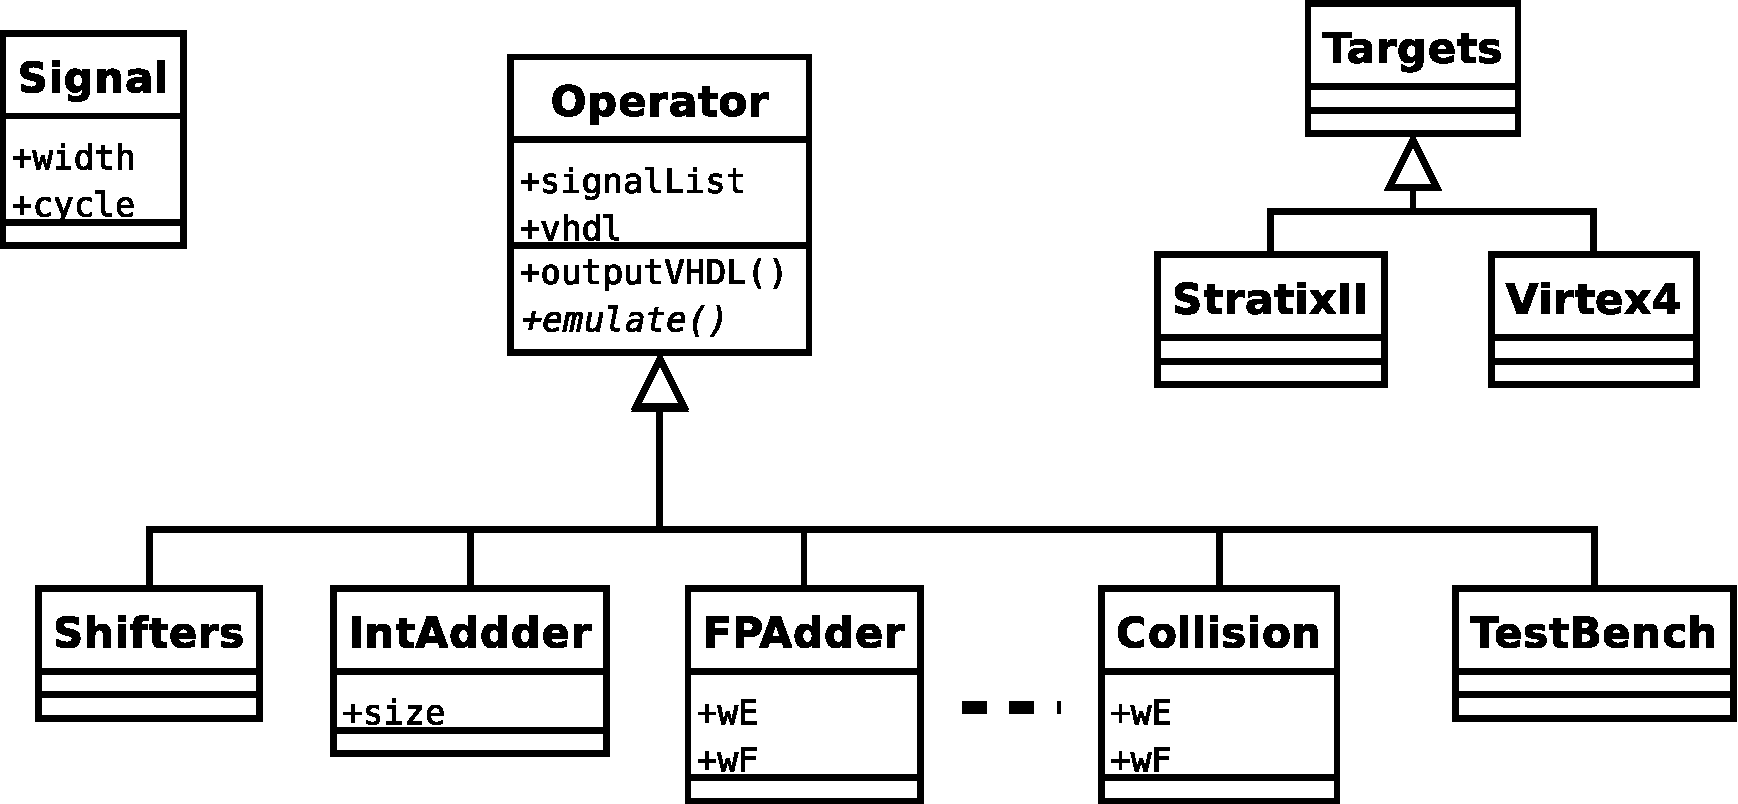
\includegraphics[width=0.7\textwidth]{../Figures/FloPoCoClasses.pdf}        
%  \end{latexonly}
\end{center}

\subsection{First steps in FloPoCo operator writing}

FloPoCo mostly requires you to embed the part of the VHDL that is between the \texttt{begin} and the \texttt{end} of the architecture
into the constructor of a class that inherits from
\verb!Operator!. The following is minimal FloPoCo code for
\verb!MAC.cpp!:
\begin{verbatim}
#include "Operator.hpp"

class MAC : public Operator
{
public:
// The constructor
MAC(Target* target): Operator(target)
{
	setName("MAC");
	setCopyrightString("ACME MAC Co, 2009");		

	// Set up the IO signals
	addInput ("X"  , 64);
	addInput ("Y"  , 32);
	addInput ("Z"  , 32);
	addOutput("R"  , 64);

   vhdl << declare("T", 64) << " <= Y * Z;" << endl;
   vhdl << "R <= X + T;" << endl;
}

// the destructor
	~MAC() {}
\end{verbatim}
 
And that's it. \verb!MAC! inherits from \verb!Operator! the method
\verb!outputVHDL()! that will assemble the information defined in the
constructor into synthesizable VHDL. Note that \verb!R! is declared by \verb!addOutput!.

So far we have gained little, except that is is more convenient to
have the declaration of \verb!T! where its value is defined. Let us
now turn this design into a pipelined one.

\subsection{Adding delay information}
A latency (in seconds) may be passed as first optional argument to  \texttt{declare()}.
  This value decribes the contribution of this VHDL statement to the critical path, and will be used to pipeline the operator (see Section~\ref{sec:pipeline} for details).
  This latency is best defined using methods of \texttt{Target}: this way the pipeline will adapt to the target.
  See \texttt{FPAddSinglePath} for examples.

\subsection{Sub-components: unique instances}

In FloPoCo, most instances are \emph{unique}: an \texttt{Operator} is built for a specific context, optimized for this context, and only one instance of this Operator will be used in the VHDL.
This is the default situation, because it allows the tool to optimize the pipelining of each component for its context.
The preferred method to use in such case is the \emph{newInstance()} method of Operator. 
See \texttt{FPAddSinglePath} for an example of a large component that instantiates many sub-components (several \texttt{IntAdder}, \texttt{Shifter}, etc).

\texttt{newInstance()} uses the factory-based user interface.
It is common to need a table of pre-computed values.
To get a unique instance of such a table,  first build the table content as a \verb!vector<mpz_class>!, then call \texttt{Table::newUniqueInstance()}.
See examples in \texttt{Trigs/FixSinCos.cpp}.


If for some reason you want to use a unique instance but don't want/need to expose a user interface for it, you just have to follow the same sequence of calls as you may find in \texttt{Table::newUniqueInstance()}.

Beware, the order is important for the operator scheduling to work properly, and it has changed since version 5.0.

\subsection{Sub-components: shared instances}

A component may also be shared (i.e. the same component is reused many times).
Simple examples are the tables in \texttt{FPConstDiv}, or in \texttt{IntConstDiv}.

The preferred method to use in such case is the \emph{newSharedInstance()} method of Operator, as in the following:
\begin{verbatim}
Operator* op = new MySubComponent(...);
op -> setShared();
//now some loop that creates many instances
for (....) {
  string myInstanceName = ...; 
  string actualX = ...;
  string actualR = ...;
  vhdl << declare(actualX, ..) << " <= " << ...;   
  newSharedInstance(op, myInstanceName, "X=>"+actualX, "R=>"+actualR);
}
\end{verbatim}

See \texttt{IntConstDiv} or \texttt{FPDiv} for detailed examples.

\subsection{Using the Table object}
Small tables of precomputed values are very powerful components, especially when targetting FPGAs.
They are quite often shared.

See \texttt{IntConstDiv} or \texttt{FPDiv} for examples of small, shared tables (intended to be implemented as LUTs on FPGAs, and as logic gates on ASIC).

See \texttt{FixFunctionByTable} for an example how to inherit \texttt{Table}.

See \texttt{FixFunctionByPiecewisePoly} for an example how to instanciate a \texttt{Table} as a sub-components.

TODO (not repaired yet): See \texttt{FPExp} for an example of unique Table intended to fit in a block RAM.




\subsection{Linking against FloPoCo\label{sec:linking}}
All the operators provided by the FloPoCo command line are available programmatically in libFloPoCo.
%A minimal example of using this library is provided in \texttt{src/main\_minimal.cpp}.

There are two ways to instantiate an operator.
One is to use its factory, which replicates the command line.

The other one is to use the constructor (whose interface is defined in the corresponding \texttt{hpp} file).
There is no one-to-one correspondance.
\begin{itemize}
\item Sometimes the command-line interface regroups several Operators.
  For instance FPAddSinglePath and FPAddDualPath are, for historical reasons, two different Operators with two different constructors, but are exposed on the interface as one FPAdd with an option.
  
\item Sometimes, the constructor has more interface options than what ends up in the command-line interface, either that some options turned out not to provide interesting solutions, or that they were
  designed for research purpose only.
\end{itemize}

\section{Test bench generation}\label{sec:test-bench-gener}

\subsection{Overview}
\texttt{\small Operator} provides one more virtual method, \texttt{\small emulate()},
to be overloaded by each Operator. As the name indicates, this method
provides a bit-accurate simulation of the operator.
 
Once this method is available, the command\\
 \texttt{flopoco FPAdd we=8 wf=23 TestBench n=500} \\
produces a test bench of 500 test vectors to exercise \texttt{\small FPAdd}. 

This test bench is properly synchronized if the operator under test happens to be pipelined: \texttt{\small emulate()} only has to specify the mathematical (combinatorial) functionality of the operator.

The \texttt{\small emulate()} method should be considered  the specification of the behaviour of the operator.
Therefore, as any instructor will tell you, it should be written \emph{before} the code generating the VHDL of the operator (test-driven design).


To see examples of \texttt{emulate()} functions, see
\begin{itemize}
\item \texttt{IntAdder} or \texttt{IntConstDiv} for an operator with integer inputs and outputs;
  For these, the GNU Multiple Precision library is your friend.
\item \texttt{FixRealKCM} for an operator with fixed-point inputs and outputs;
\item \texttt{FPAdd}  for an operator with floating-point inputs and outputs;
  For these, your friend is the GNU MPFR library, and FloPoCo provides all the needed helper functions to convert between bit vectors and MPFR numbers.
\end{itemize}


\subsection{\texttt{emulate()}  internals}
\texttt{\small emulate()} has a single argument which is a \texttt{\small TestCase}.
This is a data-structure associating inputs to outputs.
Upon entering \texttt{\small emulate()}, the input part is filled (probably by \texttt{\small TestBench}), and the purpose of \texttt{\small emulate()} is to fill the output part.
\texttt{\small emulate()} is completely generic:
Both inputs and outputs are specified as bit vectors.
However these vectors are stored for convenience in \texttt{\small mpz\_class} numbers.
This class is a very convenient C++ wrapper around GMP, which can almost be used as an \texttt{\small int}, but without any overflow issue.

Therefore an input/output is a map of the name (which should match those defined by \texttt{\small addInput} etc.) and a \texttt{\small mpz\_class}.
When the input/outputs are integers, this is a perfect match.

When the input/outputs are floating-point numbers, the most convenient multiple-precision library is MPFR.
However the I/Os  are nevertheless encoded as \texttt{\small mpz\_class}.
The \texttt{\small emulate()} method therefore typically must
\begin{itemize}
\item convert the \texttt{\small mpz\_class} inputs to arbitrary precision floating-point numbers in the MPFR format -- this is done with the help of the \texttt{\small FPNumber} class;
\item compute the expected results, using functions from the MPFR library;
\item convert the resulting MPFR number into its bit vector, encoded in an \texttt{\small mpz\_class}, before completing the \texttt{\small TestCase}. 
\end{itemize}
This double conversion is a bit cumbersome, but may be copy-pasted from one existing operator: Imitate \texttt{\small FPAddSinglePath} or \texttt{\small FPExp}.


\subsection{Fully and weakly specified operators}
 Most operators should be fully specified: for a given input
  vector, they must output a uniquely defined vector. This is the case of 
  \texttt{\small IntAdder} above. For floating-point
  operators, this unique output is the combination of a mathematical
  function and a well-defined rounding mode. The bit-exact MPFR
  library is used in this case. Imitate \texttt{\small FPAddSinglePath} in this case.

 Other operators are not defined so strictly, and may have  several acceptable output values.
 The last parameter of \texttt{\small addOutput} defines how many values this output may take.
 An common requirement is \emph{faithful rounding}: the operator should return one of the two FP values surrounding the exact result\footnote{
 The allowed error is twice as large as correct rounding, so a correctly rounded result on $p$ bits is as accurate as a faithful result on $p+1$ bits. 
 However, (for reasons too long to detail here) a faithful operator may be much, much cheaper to build than a correctly rounded one.
 In such cases it is cheaper to build a faithful operator to $p+1$ bits than a correctly rounded one to precision $p$.}
These values may be obtained thanks to the  \emph{rounding up} and \emph{rounding down} modes supported by MPFR.
See \texttt{\small FPExp} or \texttt{\small FPLog} for  examples in floating point, and \texttt{FixSinCos} for an example in fixed point (which is also an example where the function has two outputs).

\subsection{Operator-specific test  vector generation}
Overloading \texttt{\small emulate()} is enough for FloPoCo to be able
to create a generic test bench using random inputs. The default random generator is uniform over the input bit vectors. It is
often possible to perform better, more operator-specific test-case
generation. Let us just take two examples.

\begin{itemize}\item 
  A double-precision exponential returns $+\infty$ for all inputs
  larger than 710 and returns $0$ for all inputs smaller than
  $-746$. In other terms, the most interesting test domain for this
  function is when the input exponent is between $-10$ and $10$, a
  fraction of the full double-precision exponent domain ($-1024$ to
  $1023$). Generating uniform random 64-bit integers and using them as
  floating-point inputs would mean testing mostly the
  overflow/underflow logic, which is a tiny part of the operator.


\item In a floating-point adder, if the difference between the
  exponents of the two operands is large, the adder will simply return
  the biggest of the two, and again this is the most probable
  situation when taking two random operands. Here it is better to
  generate random cases where the two operands have close
  exponents. Besides, a big part of the adder architecture is
  dedicated to the case when both exponents differ only by 1, and
  random tests should be focused on this situation.
\end{itemize}
Such cases are managed by overloading the Operator method  \texttt{\small buildRandomTestCases()}. 
See \texttt{FPExp.cpp} and \texttt{FPAdd.cpp} for the examples above.

\subsection{Corner-cases and regression tests}
Finally, \texttt{\small buildStandardTestCases()} allows to test corner cases which random testing has little chance to find.
See \texttt{\small FPAdd.cpp} for examples. 

Here, it is often useful to add a comment to a test case using \texttt{\small addComment}: these comments
will show up in the VHDL generated by \texttt{\small TestBench file=false}.


\subsection{Regression testing, build test }
The command \verb!flopoco Autotest Operator=FPadd! tests FPAdd for a range of relevant parameter values.
For each parameter vector, it reports if the FloPoCo command succeeded, if the VHDL was syntactically correct, and if the simulation of this VHDL was successful.

The enumeration of the parameter vectors is defined in the (optional) static method \texttt{FPAdd::unitTest()}.
This is a relatively recent addition to the framework, and not all operators support it, but it is strongly advised to set it up in the early steps of operator development: it helps uncover bugs that occur for specific values of the parameters.

The command \verb!flopoco Autotest Operator=all! runs this test for all the operators that support it.
It may take long...




\section{Frequency-directed pipeline \label{sec:pipeline}}

The  pipeline framework  is implemented mostly in the \texttt{Operator} and \texttt{Signal} classes, and we refer the reader to the source code for the full  details.
More details can also be found in \cite{istoan:hal-01373937}.

\subsection{VHDL generation for a simple component}

\subsubsection{First VHDL parsing and signal graph construction}
The \texttt{vhdl} stream is parsed (as the constructor writes to it) to locate VHDL signal identifiers.

This pass builds  a signal graph, an example of which is shown on Figure~\ref{fig:depgraphShifter} 
(it was obtained in \texttt{flopoco.dot} by the command
\verb!./flopoco Shifter wIn=8 maxshift=8 dir=1! )

In this graph, the nodes are signals (of the FloPoCo \texttt{Signal} class), and the edges are signal dependencies, \emph{i.e.} which signal is computed out of which signal.
Technically, the graph is built by defining predecessors and successors of each \texttt{Signal}.

The operations between the signals are not kept in this graph: they are kept in the \texttt{vhdl} stream.
  However, their latency (passed as first optional argument to  \texttt{declare()}) is used to label each signal.
  This value decribes the contribution of this VHDL statement to the critical path.

  In Figure~\ref{fig:depgraphShifter}, the first line of each box is the signal name.
The second line is the critical path contribution of each signal.
  The third line is the actual global timing of each signal, which is computed in the following. 
  
The reader interested in this first parsing pass should have a look at \texttt{FlopocoStream.cpp}.

  \begin{figure}
    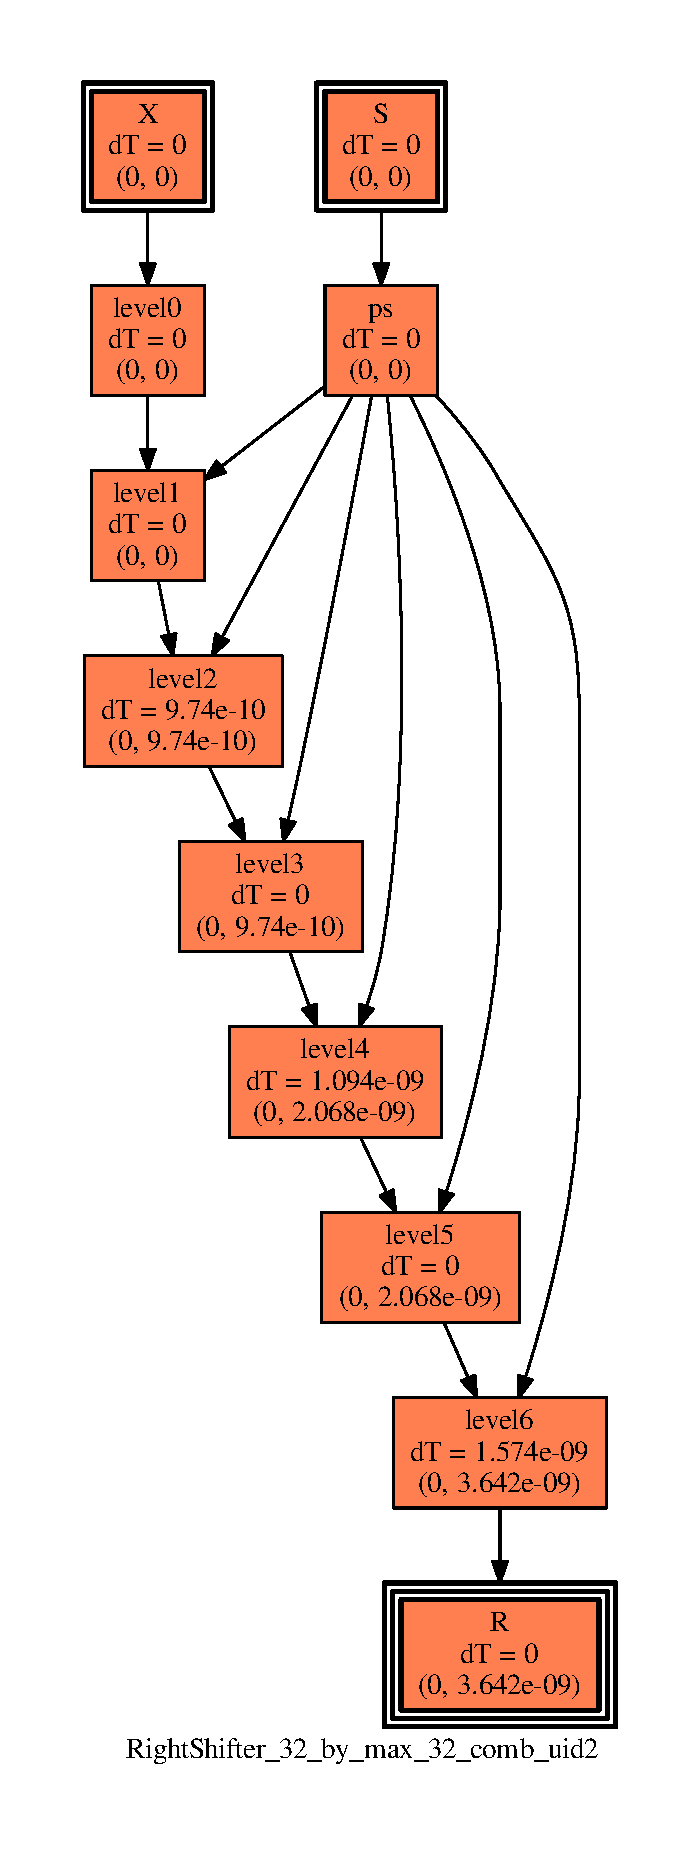
\includegraphics[width=0.4\textwidth]{Fig/depgraphShifterNoPipe}
    \hfill
    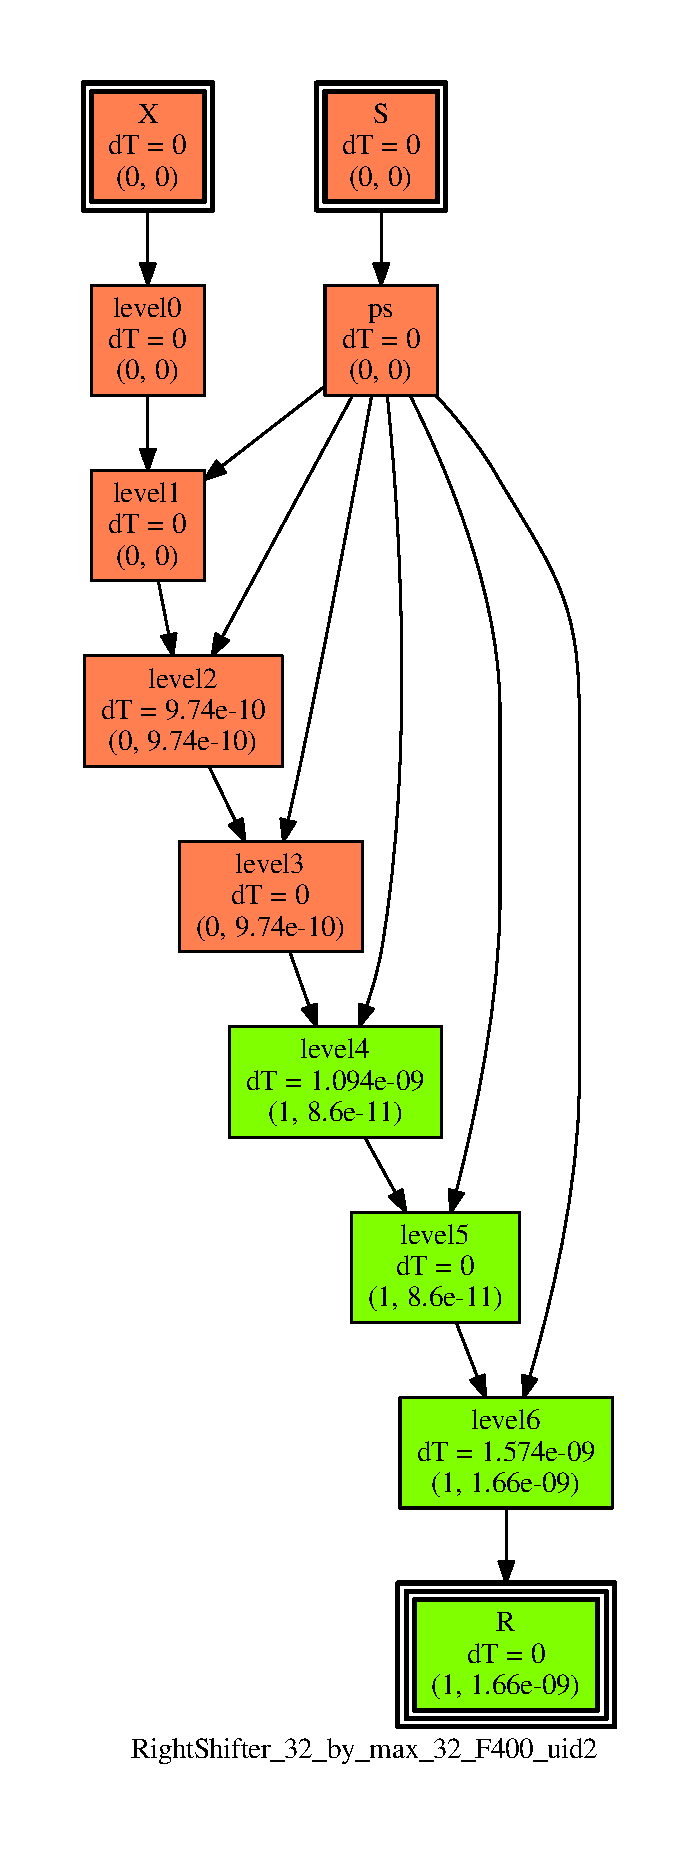
\includegraphics[width=0.4\textwidth]{Fig/depgraphShifterPipelined}
		\centering
		\caption{S-Graph for a combinatorial 8-bit barrel shifter, combinatorial (left) and pipelined (right)}
		\label{fig:depgraphShifter}
	\end{figure}    


\subsubsection{Scheduling of the signal graph}\label{sec:scheduling}
The second step of automatic pipelining is the scheduling of the signal graph.
It is implemented in the method \texttt{Operator::schedule()}.
It is an ASAP (as soon as possible) scheduling: starting from the input, we accumulate the critical path along the edges of the signal graph.

With the \texttt{pipeline=no} option, what we obtain in \texttt{flopoco.dot} is an estimate of the critical path from an input to each signal.


With \texttt{pipeline=yes}, the schedule constructs a pipeline.
Each signal is assigned a cycle and a critical path within this cycle (i.e. what we obtain in \texttt{flopoco.dot} is an estimate of the critical path from the output of a register to each signal.

The timing of a signal is therefore expressed as a pair $(c, \tau)$, where
\begin{itemize}
\item $c$ is an integer that counts the number of registers
  on the longest path from an input to $s$.
\item $\tau$ is a real number that represents the critical path delay (in seconds)
  from the last register or earliest input to $s$.
\end{itemize}

The colors on Fig. \ref{fig:depgraphShifter}, right,  indicate the cycle.
The complete lexicographic time of each signal is given by the third line of each signal box. 

There is a lexicographic order on such timings: $(c_1, \tau_1) > (c_2, \tau_2)$ if $c_1 > c_2$ or if $c_1 = c_2$ and $\tau_1 > \tau_2$.

\subsubsection{Back-annotation of the VHDL stream with delay information}
Once each signal is scheduled, there is a second parsing step of the VHDL stream that delays each signal where it is needed by the proper number of cycle.
Technically, when parsing
\verb!A <= B and C;!, the schedule has ensured that  \verb!B.cycle!$\le$ \verb!A.cycle!.
If \verb!A.cycle! $>$ \verb!B.cycle!, FloPoCo delays
signal \verb!B! by n=\verb!A.cycle! $-$ \verb!B.cycle! cycles.

Technically, it just replaces, in the output VHDL,   \verb!B! with \verb!B_dn!.
It also updates bookkeeping information that gives the life span of each signal.

This process is performed by the \verb!Operator::applySchedule()! method.

\subsubsection{Final VHDL output}
The final step adds to the VHDL stream constructed from previous step all the declarations (entities, signals, etc) as well as the shift registers that delay signals.
It is performed by the \verb!Operator::outputVHDL()! method.

\subsection{Subcomponents and instance}

Now consider the more complex situation of a component that include other subcomponents.
There are two distinct situations:
\begin{itemize}
\item either the subcomponent is used only once, in which case we want to schedule it in its context.
  This is the default situation.
  An extensive example of a complex component built by assembling simpler ones is \texttt{FPAddSub/FPAddSinglePath}.
  
\item Or, the subcomponent is used many times (a typical example is the compressor in a bit heap), in which case all the instances will necessarily share the same schedule.
  In FloPoCo, we add a constraint in this case: such operators remain very small and thus shall not be pipelined.
  This covers 100\% of the use cases so far.
  Such components have to be declared shared by calling \texttt{Operator::setShared()}.
\end{itemize}

In the following we detail these two cases and what happens under the hood in terms of scheduling.


\subsubsection{Unique instances}
In this case, the entity of the subcomponent is used in only one VHDL instance.

FloPoCo provides for this case a single method, \verb!Operator::newInstance()!.
Its inputs are those provided on the command-line interface, therefore this method will only work for operators which implement the factory methods.
It returns a pointer to the newly created \texttt{Operator}.

In terms of VHDL, \verb!Operator::newInstance()! creates both the entity of the subcomponent (by calling its constructor) and an instance of this entity in the \texttt{vhdl} stream of the current buffer.

Let us now see what happens in terms of scheduling and pipelining.
\begin{itemize}
\item In the signal graph, \verb!Operator::newInstance()! connects the actual signals to the subcomponent ports, with simple wires (no delay added to the critical path).
  The \texttt{flopoco.dot} output shows a box around the signals of the subcomponent, but there is one single graph linking \texttt{Signal} objects.

\item It is useful that the constructor of the subcomponent may take decisions based on the schedule of its inputs (example: the \texttt{IntAdder} pipelined integer splits its inputs depending on their critical path).
  Therefore, \verb!Operator::newInstance()! calls \verb!Operator::schedule()! (step \ref{sec:scheduling} above).

  Since there is only one big signal graph, \verb!Operator::schedule()! first gets to the root of the component hierarchy, before actually computing the schedule, starting from the inputs of this root.

\item When the inputs to a sub-component are not synchronized, they will be synchronized inside the sub-component.

\item It is important to understand that \verb!Operator::schedule()! can be invoked on an incomplete graph.
  In such an ASAP scheduling, the schedule of a signal is only defined by the schedule of its predecessors: once it is computed, it will no longer change, so \verb!Operator::schedule()! may be called several times. It will be called by default after the end of the constructor of a root operator (so the signal graph is complete).

\item All this probably works best (only works?) if the VHDL is written in the natural order, from inputs to outputs... 

\end{itemize}


  \begin{figure}
    
\includegraphics[height=\textheight]{Fig/depgraphFPAddPipelined}
		\centering
		\caption{S-Graph for a pipelined FPAddSinglePath operator. Zoom on the Shifter component and observe that it has been pipelined for its context.}
		\label{fig:depgraphFPAdd}
	\end{figure}    



\subsubsection{Shared instances}

Again, shared instances are small, purely combinatorial components.

Here are the main differences:
\begin{enumerate}
\item The constructor of the subcomponent must be called only once.
\item The instances themselves must be somehow replicated in the signal graph.
\end{enumerate}
The solution chosen is to replace \emph{in the signal graph} instances with links between the inputs and outputs.
Each output is labeled with a critical path contribution,   equal to the critical path of this output in the instance.

This is performed under the hood by the \verb!Operator::inPortMap()!, \verb!Operator::outPortMap()! and \verb!Operator::instance()! methods.

An instance is combinatorial, hence lives within a single cycle.
Therefore, all the outputs of a shared instance have this same cycle.
All the inputs are also input at this same cycle to the instance (they are delayed in the \texttt{port map}.
If a pipeline register is inserted to account for the delay of a shared instance, it is inserted on the outputs.

The simplest example of shared instances is currently \texttt{FPDivSqrt/FPDiv}.


\subsection{Limitations of the pipelining framework}

The parser has some limitations when parsing the generated \texttt{vhdl}. The following statements are not supported:
\begin{itemize}
	\item \texttt{case} statements are not supported. Use conditional assignments (like the \texttt{with ... select} or \texttt{when} statements) if possible or \texttt{if}/\texttt{then}/\texttt{else} statements.
	\item Assignments to parts of a vector like
	
\texttt{signal v: std\_logic\_vector(1 downto 0);}\\
\texttt{(...)}\\
\texttt{v(0)<=expr1;}\\
\texttt{v(1)<=expr2;}\\
are not supported. It should be written \texttt{v <= expr2 \& expr1;} instead.
	
\end{itemize}



\section{Bit heaps \label{sec:bitheap}}

The main interface to the developer is the  \texttt{BitHeap} class, which encapsulates all the needed data structures and methods. 
The bits to be added to a \texttt{BitHeap} are simply  signals of the operator being generated.
This makes it possible to define the initial bit heap, which can be of any shape or size. 
The \texttt{BitHeap} class also implements the compressor tree optimization techniques presented in \cite{DinIstSer2013-FPL-BitHeap,kz14a,kz14b,kk18} (the compression algorithm is selected on the command line), and can generate the corresponding hardware.


%dynamical data structure that evolves during the circuit generation process.

The typical code to generate the architecture of an operator involving a bit heap is shown in Listing~\ref{algo:code-bitheap}.
The main methods to manipulate the bit heap are shown in Table~\ref{tab:bit_heap_interface}.
Basically, there is everything to add or subtract single bits, signed or unsigned numbers held in bit vectors, or constants. 
Once all the bits have been thrown on the bit heap, the \texttt{startCompression()} method launches the optimization of the compressor tree as well as the VHDL code generation.


\lstset{language=C++,numbers=none,basicstyle=\small\ttfamily,xleftmargin=5pt,xrightmargin=0pt,frame=lines,rulesepcolor=\color{black},keywordstyle=\color{black}\bfseries,escapeinside={(*}{*)},belowskip=-10pt}

\begin{lstlisting}[float, caption=Typical code for an operator involving a bit heap, label=algo:code-bitheap]
bh = new BitHeap(...);  // create an empty bit heap

// construction of the bit heap
for (...) {
  // generate VHDL that defines signals such as
  ///  mySingleBit or myBitVector
  ...
  
  // then add these signals to the bit heap: 
  bh->addBit(myBit, pos1); // no VHDL generation here 
  bh->addSignal(mybitVector, pos2); // nor here
}

// generate the compressor tree for the bit heap
bh->startCompression(); // this line generates a lot of VHDL
\end{lstlisting}


Some operators that use the BitHeap have two constructors:
\begin{itemize}
	\item one standalone, classical; The BitHeap is constructed in the operator and used only for this operator
	\item one virtual; a BitHeap from another operator is provided that is shared among the operators (which can build a more complex operator).
\end{itemize}

In the latter case, the typical arithmetic flow requires to first perform some error analysis to determine a number of guard bits to add to the bit heap.
This must be done before any VHDL generation.
If we want to delegate some of this error analysis to the subcomponents, then either it must be implemented in some static method of the Operator, or the constructor must delay the actual VHDL output to another method.

For an example of this in practice, see \texttt{FixFilters/FixSOPC}.

\begin{table}[t]
  \centering
    \begin{center}
      \caption{The main methods of the \texttt{BitHeap} interface}
	\label{tab:bit_heap_interface}
  \footnotesize
  
    \begin{tabular}{L{0.5\textwidth}L{0.4\textwidth}}
    	\toprule
		Method                                        & Description                                      \\
    	\midrule
      {\texttt{void addBit(string sigName,int pos)}}      & Add a single bit                                 \\
      {\texttt{void addSignal(string sigName,int shift)}}   & Add a fixed-point signal, with sign extension if needed                       \\
      {\texttt{void subtractSignal(string name,int shift)}} & Subtract a fixed-point signal, with sign extension if needed                  \\
      {\texttt{void addConstantOneBit(int pos)}}  & Add a constant one bit                           \\[1ex]
      {\texttt{void addConstant(mpz\_class cst,int pos)}} & Add the constant $\mathtt{cst}\cdot 2^{\mathtt{pos}}$ \\
      {\texttt{void startCompression()}}          & Generate a compressor tree                       \\
    	\bottomrule
    \end{tabular}
        When the argument is a signal name, it is used to refer to a FloPoCo object of the class Signal, which encapsulate a fixed-point format with its  signedness, its MSB, and its LSB.
    \end{center}
\end{table}



\subsection{The data structure}
This section and the following describe the internals of the \texttt{BitHeap} class, and are intended for developers wishing to extend the BitHeap framework itself (e.\,g., with new compressors or compression algorithms).

A \emph{weighted bit} is a data structure consisting essentially of a signal name, a bit position, and various fields used when building the compressor tree.
In FloPoCo the \texttt{Signal} class also encapsulates the timing of each signal, so each weighted bit also carries its arrival time.


A column of the bit heap is represented as a list of weighted bits.
This list is  sorted by the  arrival time of the bits, so that compression algorithms can compress first the bits arrived first.

The complete bit heap data structure essentially consists of its MSB and LSB, and an array of columns indexed by the positions. 

The \texttt{BitHeap} class also offers methods to visualize a bit heap as a dot diagram like the one shown in Figure~\ref{fig:bitheapgallery-halfsine}.
Use the \texttt{generateFigures} flag to enable the output of \texttt{SVG} and \texttt{.tex} files (these use the macros found in \texttt{dot\_diag\_macros.tex}).
Different arrival times may be indicated by different colors.

FloPoCo may generate such figures as SVG files that can be opened in a browser, in which case hovering the mouse over one bit shows its signal name and its arrival instant in circuit time.  
%Bits are inserted in the bit heap at the proper instant in the circuit time. This evolution of the bit heap in  should not be confused with the evolution of the bit heap in the circuit time. 

%It should be clear that there are two aspects of time here: operator-generation time (as the generator program runs), and circuit time (using notions such as critical path or, for pipelined designs, cycles). 
%The generator must be able to evaluate the circuit time, for instance as in \cite{DinechinPasca2011-DaT}.

\begin{figure}[t]
  \centering
    % obtained directly from FloPoCo
    % $ ./flopoco FixHalfSine lsbIn=-16 lsbout=-16 n=4
    \scalebox{0.28} {
      \begin{dotdiag}{20}
        \begin{scope}
          \drawdotcol{0}{16}
          \drawdotcol{1}{16}
          \drawdotcol{2}{16}
          \drawdotcol{3}{16}
          \drawdotcol{4}{14}
          \drawdotcol{5}{12}
          \drawdotcol{6}{12}
          \drawdotcol{7}{12}
          \drawdotcol{8}{12}
          \drawdotcol{9}{10}
          \drawdotcol{10}{8}
          \drawdotcol{11}{8}
          \drawdotcol{12}{8}
          \drawdotcol{13}{8}
          \drawdotcol{14}{6}
          \drawdotcol{15}{4}
          \drawdotcol{16}{4}
          \drawdotcol{17}{4}
          \drawdotcol{18}{4}
          \drawdotcol{19}{3}
        \end{scope}
      \end{dotdiag}
    }
  \caption{Bit heap obtained for a 16-bit, 8-tap half-sine pulse shaping FIR filter operator \texttt{FixHalfSine}}
  \label{fig:bitheapgallery-halfsine}
\end{figure}

\subsection{Compressor tree generation}

Once the data structure of the BitHeap is created by using the methods of Table~\ref{tab:bit_heap_interface}, the compressor tree generation is started by calling \texttt{startCompression()}.
It involves the following steps:
\begin{enumerate}
	\item The algorithm for solving the compressor tree problem is selected (a derived class from \texttt{CompressionStrategy}).
	\item A list of possible (target-dependent) compressors is generated (class \texttt{BasicCompressor} for representing the shape and class \texttt{Compressor} implementing the Operator performing the compression).
	\item Then, the bits of the bit heap are scheduled to different stages according to their cycle and combinatorial arrival time.
	\item Next, the compressor trees are optimized (by a class derived from \texttt{CompressionStrategy}) and a \texttt{BitHeapSolution} object is created. This solution contains the used compressors per stage and column.
	\item Finally, the VHDL code of the compressor tree is generated.
\end{enumerate}

New compressor tree optimization methods can be implemented  by extending \texttt{CompressionStrategy}.



\section{Writing a new target}
Try to fill data such as LUT input size (\texttt{lutInputs()}), etc.

Here are some operators that can be used to calibrate delay functions.
You may use the scripts in \texttt{tools/} to launch syntheses and get critical path reports.
It is better to ask for a relatively low frequency (say, half peak, 200MHz) to avoid troubles with I/O buffer delays when using post place-and-route synthesis.

\begin{itemize}
\item To calibrate the logic delay, use 
\begin{verbatim}
  ./flopoco IntConstDiv wIn=64 d=3 Wrapper
\end{verbatim}
  If you have specified your lutInputs properly, the architecture should be a sequence of LUTs connected by local routing.
  First check that the estimated cost reported by FloPoCo matches the actual cost. 
  
\item To calibrate the IntAdder delay, use
\begin{verbatim}
  ./flopoco IntAdder wIn=64 Wrapper
\end{verbatim}
  for increasing values of 64.
  
\end{itemize}


\bibliographystyle{IEEEtran}
% argument is your BibTeX string definitions and bibliography database(s)
\bibliography{../web/bib/flopoco.bib,../web/bib/flopoco-users.bib,flopoco_manual.bib}

\end{document}
